% !Mode:: "Tex:UTF-8"



\documentclass[10pt,a4paper]{article}\usepackage[]{graphicx}\usepackage[]{color}
%% maxwidth is the original width if it is less than linewidth
%% otherwise use linewidth (to make sure the graphics do not exceed the margin)
\makeatletter
\def\maxwidth{ %
  \ifdim\Gin@nat@width>\linewidth
    \linewidth
  \else
    \Gin@nat@width
  \fi
}
\makeatother

\definecolor{fgcolor}{rgb}{0.345, 0.345, 0.345}
\newcommand{\hlnum}[1]{\textcolor[rgb]{0.686,0.059,0.569}{#1}}%
\newcommand{\hlstr}[1]{\textcolor[rgb]{0.192,0.494,0.8}{#1}}%
\newcommand{\hlcom}[1]{\textcolor[rgb]{0.678,0.584,0.686}{\textit{#1}}}%
\newcommand{\hlopt}[1]{\textcolor[rgb]{0,0,0}{#1}}%
\newcommand{\hlstd}[1]{\textcolor[rgb]{0.345,0.345,0.345}{#1}}%
\newcommand{\hlkwa}[1]{\textcolor[rgb]{0.161,0.373,0.58}{\textbf{#1}}}%
\newcommand{\hlkwb}[1]{\textcolor[rgb]{0.69,0.353,0.396}{#1}}%
\newcommand{\hlkwc}[1]{\textcolor[rgb]{0.333,0.667,0.333}{#1}}%
\newcommand{\hlkwd}[1]{\textcolor[rgb]{0.737,0.353,0.396}{\textbf{#1}}}%

\usepackage{framed}
\makeatletter
\newenvironment{kframe}{%
 \def\at@end@of@kframe{}%
 \ifinner\ifhmode%
  \def\at@end@of@kframe{\end{minipage}}%
  \begin{minipage}{\columnwidth}%
 \fi\fi%
 \def\FrameCommand##1{\hskip\@totalleftmargin \hskip-\fboxsep
 \colorbox{shadecolor}{##1}\hskip-\fboxsep
     % There is no \\@totalrightmargin, so:
     \hskip-\linewidth \hskip-\@totalleftmargin \hskip\columnwidth}%
 \MakeFramed {\advance\hsize-\width
   \@totalleftmargin\z@ \linewidth\hsize
   \@setminipage}}%
 {\par\unskip\endMakeFramed%
 \at@end@of@kframe}
\makeatother

\definecolor{shadecolor}{rgb}{.97, .97, .97}
\definecolor{messagecolor}{rgb}{0, 0, 0}
\definecolor{warningcolor}{rgb}{1, 0, 1}
\definecolor{errorcolor}{rgb}{1, 0, 0}
\newenvironment{knitrout}{}{} % an empty environment to be redefined in TeX

\usepackage{alltt}
\usepackage{etoolbox}
\newtoggle{color}
%\togglefalse{color}
\toggletrue{color}

\usepackage{makeidx}
\newcommand{\idioma}{spanish}
\newcommand{\opcionesIdioma}{,es-nodecimaldot,es-tabla}
% !Mode:: "Tex:UTF-8"
%%%%%%%%%%%%%%%%%%%%%Carga de Packages
%%poner \newcommand{\idioma}{spanish} o \newcommand{\idioma}{english} en el documento
\usepackage{pdfsync}
\usepackage{srcltx}
\usepackage[\idioma\opcionesIdioma]{babel}
\usepackage[utf8x]{inputenc}
\usepackage[T1]{fontenc}
\usepackage{graphicx}
\graphicspath{{/users/fernando/figuras/}{./}{./figuras/}{/fernando/figuras/}{/fernando/figuras/jpg/}}
\usepackage{multicol}
\usepackage{epsfig}
%\usepackage{oberdiek}
\usepackage{listingsutf8}
\lstset{inputencoding=utf8/latin1}
%\lstset{extendedchars=true}
\lstset{ %
  language=R,                     % the language of the code
  basicstyle=\ttfamily\small,       % the size of the fonts that are used for the code
  numbers=left,                   % where to put the line-numbers
  numberstyle=\tiny\color{gray},  % the style that is used for the line-numbers
  stepnumber=1,                   % the step between two line-numbers. If it's 1, each line
                                  % will be numbered
  numbersep=5pt,                  % how far the line-numbers are from the code
  backgroundcolor=\color{white},  % choose the background color. You must add \usepackage{color}
  showspaces=false,               % show spaces adding particular underscores
  showstringspaces=false,         % underline spaces within strings
  showtabs=false,                 % show tabs within strings adding particular underscores
  frame=single,                   % adds a frame around the code
  rulecolor=\color{black},        % if not set, the frame-color may be changed on line-breaks within not-black text (e.g. commens (green here))
  tabsize=2,                      % sets default tabsize to 2 spaces
  %captionpos=,                   % sets the caption-position to bottom
  breaklines=true,                % sets automatic line breaking
  breakatwhitespace=false,        % sets if automatic breaks should only happen at whitespace
  %title=\lstname,                 % show the filename of files included with \lstinputlisting;
                                  % also try caption instead of title
  keywordstyle=\color{black},      % keyword style
  commentstyle=\color{Brown},   % comment style
  stringstyle=\color{black},      % string literal style
  escapeinside={\%*}{*)},         % if you want to add a comment within your code
  morekeywords={*,...},            % if you want to add more keywords to the set
  lineskip={-2.5pt} % single line spacing
}
%\usepackage{algorithm}
\usepackage{amsmath}
\usepackage{amsfonts}
\usepackage{amssymb}
\usepackage{amsthm}
\usepackage{fancybox}
\usepackage{fancyvrb}
\usepackage{rotating}
\usepackage{keystroke}
\usepackage{array}
\input{xy}
\xyoption{all}
%\usepackage[dvipsnames,usenames]{color}
\usepackage[usenames,dvipsnames,svgnames,table]{xcolor}
\usepackage{colortbl}
\usepackage{comment}
\excludecomment{spanish}
\excludecomment{english}
\includecomment{\idioma}

%\usepackage{noweb}
%\usepackage{clrscode}
\usepackage{eurosym}
\usepackage{wasysym}
\usepackage{multirow}
%\usepackage{margins}
\usepackage{lscape}
\usepackage{longtable}
\usepackage[normalem]{ulem}
\usepackage{xr-hyper}

%%NUEVO
\newcolumntype{C}{{\centering\arraybackslash}m{20mm}}
\newcommand{\centercell}[1]{\multicolumn{1}{c}{#1}}
\newcommand{\colHead}[1]{\centercell{\bfseries#1}}

\excludecomment{ocultar}


% Matriz (par‚ntesis)
\def\matr#1#2{\left(\begin{array}{#1}#2\end{array}\right)}
% Determinante (barras)
\def\deter#1#2{\left|\begin{array}{#1}#2\end{array}\right|}
% Sistema de ecuaciones. (llave a la izda.)
\def\seq#1#2{\left\{\begin{array}{#1}#2\end{array}\right.}
% Ecuaci\'on de varias lineas (sin llave a la izda.)
\def\evl#1#2{\begin{array}{#1}#2\end{array}}

%%%%%%%%%%%%%%%%%%%%%%%%%%%%%%%%%%%%%%%%%%%%%%
%%%%%%%%%%%%%%%%%%%%%%%%%%%%%%%%%%%%%%%%%%%%%%
%%%%%%%%%%%%%%%%% M\'{a}rgenes %%%%%%%%%%%%%%%%
%
%
%\parindent=0mm
%
%\textwidth=160mm
%\textheight=220mm
%\hoffset=-20mm
%\voffset=-15mm
%\parskip=0mm
\marginparsep=3mm
\marginparwidth=25mm
%
%%%%%%%%%%%%%%%%%%%%%%%%%%%% Contadores para listas de problemas
%\newcommand{\adc}{\addtocounter{enumi}{1}}
\newcommand{\adc}{\stepcounter{enumi}}
\newcommand{\adci}{\stepcounter{enumii}}
\newcommand{\xadc}{\addtocounter{xcounter}{1}}
\newcommand{\be}{\begin{enumerate}}
\newcommand{\ee}{\end{enumerate}}
\newcommand{\bi}{\begin{itemize}}
\newcommand{\ei}{\end{itemize}}
\newcounter{xcounter}


\newcommand{\nin}{{\noindent}}

%\newcounter{prob}{}
%\def\pr{\addtocounter{prob}{1}(\theprob)\ }
%\def\pr2{\addtocounter{prob}{2}(\theprob)\ }

%%%%%%%%%%%%%%%%%%%%%%%%%%%Fin de demostraciones, ejemplos, etc.
\newcommand{\fin}{$\square$}
%%%%%%%%%%%%%%%%%%%%%%%%%%Notaci\'{o}n matem\'{a}ticas generales
%\newcommand{\suc}[1]{\{#1_n\}}
%\newcommand{\sucn}[1]{\{#1_n\}_{n\in\mathbb{N}}}
%\newcommand{\ser}[1]{\sum #1_n}
%\newcommand{\sern}[1]{\sum_{n\geq 1} #1_n}
%\newcommand{\limn}{\lim_{n\rightarrow\infty}}
%\newcommand{\limnd}{\displaystyle\lim_{n\rightarrow\infty}}
%\newcommand{\mf}[1]{\mathbf{#1}}
%\newcommand{\mb}[1]{\mathbb{#1}}
%\newcommand{\D}[1]{\Dv_{\mf{#1}}}
%\newcommand{\bsigma}{\pmb{\sigma}}
%\newcommand{\bPhi}{\pmb{\Phi}}
%\newcommand{\vol}{\operatorname{vol}}
%\newcommand{\ldbr}{[\hspace{-1.5pt}[}
%\newcommand{\rdbr}{]\hspace{-1.5pt}]}
%\newcommand{\fpws}[2]{{#1}\ldbr{#2}\rdbr}
%\newcommand{\leftPui}{<\hspace{-3pt}<}
%\newcommand{\rightPui}{\hspace{-3pt}}
%\newcommand{\Pui}[2]{{#1}\hspace{-6pt}\leftPui{#2}\rightPui}
%\newcommand{\pdd}[2]{\dfrac{\partial{#1}}{\partial{#2}}}
%%%%%%%%%%Conjuntos de n\'{u}meros
\newcommand{\N}{\mathbb{N}} %conjunto de n\'{u}meros naturales
\newcommand{\Z}{\mathbb{Z}} %conjunto de n\'{u}meros enteros
\newcommand{\R}{\mathbb{R}} %conjunto de n\'{u}meros reales
\newcommand{\C}{\mathbb{C}} %conjunto de n\'{u}meros complejos
\newcommand{\Q}{\mathbb{Q}} %conjunto de n\'{u}meros racionales
\newcommand{\EP}{\mathbb{P}} %espacios proyectivos
\newcommand{\K}{\mathbb{K}} %cuerpo gen\'{e}rico
\newcommand{\A}{\mathbb{A}} %espacios afines

%%%%%%%%%%Estadistica
\newcommand{\MEAN}{\mathrm{E}}
\newcommand{\Var}{\mathrm{Var}}
\newcommand{\Cov}{\mathrm{Cov}}


%%%%%%%%%%Funciones
\def\arcsen{\operatorname{arcsen}}
\def\arctg{\operatorname{arctg}}
\def\argCosh{\operatorname{argCosh}}
\def\argSenh{\operatorname{argSenh}}
\def\argTgh{\operatorname{argTgh}}
\def\cosec{\operatorname{cosec}}
\def\Cosh{\operatorname{Cosh}}
\def\cotg{\operatorname{cotg}}
\def\Dv{\operatorname{D}}
\def\discrim{\operatorname{discrim}}
\def\dive{\operatorname{div}}
\def\dom{\operatorname{dom}}
\def\Ext{\operatorname{Ext}}
\def\Fr{\operatorname{Fr}}
\def\dder#1#2{\dfrac{d #1}{d #2} } %derivada en estilo display
\def\gr{\operatorname{gr}}
\def\grad{\operatorname{grad}}
\def\Imag{\operatorname{Im}}
\def\mcm{\operatorname{mcm}}
\def\rang{\operatorname{rang}}
\def\rot{\operatorname{rot}}
\def\sen{\operatorname{sen}}
\def\Senh{\operatorname{Senh}}
\def\sgn{\operatorname{sgn}}
\def\sig{\operatorname{sig}}
\def\tg{\operatorname{tg}}
\def\Tgh{\operatorname{Tgh}}
\def\E{\operatorname{E}}
\def\VAR{\operatorname{VAR}}
\newcommand{\margWeb}[2]{\noindent{#2}\marginpar[\hspace{-18mm}\link{#1}{WEB}]{\hspace*{-18mm}\link{#1}{WEB}}}

%%%%%%%%%%%%%%%%%%%%%%\'{A}lgebra conmutativa.
\def\multideg{\operatorname{multideg}} %multidegree of a polynomial
\def\LT{\operatorname{lt}} %leading term of a polynomial
\def\LC{\operatorname{lc}} %leading coefficient of a polynomial
\def\LM{\operatorname{lm}} %leading monomial of a polynomial
\def\Mexp{\mathbb{Z}^n_{\geq 0}} %set of multiexponents of monomials
\def\set#1{\left\{{#1}\right\}}
\newcommand{\vlist}[2]{\mbox{${#1}_{1},\ldots,{#1}_{#2}$}}
\def\deg{\operatorname{deg}} %grado de un polinomio
\def\cp{\operatorname{cp}} %coeficiente principal de un polinomio
\def\CP{\operatorname{cp}} %coeficiente principal de un polinomio
\def\set#1{\left\{{#1}\right\}} %llaves de conjunto
\newcommand{\V}{{\bf V}} %variedad de un conjunto de polinomios
\newcommand{\I}{{\bf I}} %ideal de un conjunto
\newcommand{\MCD}{\operatorname{mcd}} %m\'{a}ximo com\'{u}n divisor
\newcommand{\MCM}{\operatorname{mcm}} %m\'{\i}nimo com\'{u}n m\'{u}ltiplo
\newcommand{\LCM}{\operatorname{lcm}} %least common multiple
\newcommand{\GCD}{\operatorname{gcd}} %greatest common divisor
\newcommand{\Ker}{\operatorname{Ker}} %N\'{u}cleo
\newcommand{\IM}{\operatorname{IM}} %Imagen
\newcommand{\Rad}{\operatorname{Rad}} %radical de un ideal
\newcommand{\Jac}{\operatorname{Jac}} %radical de Jacobson de un anillo
\newcommand{\Ann}{\operatorname{Ann}} %anulador de un ideal
\newcommand{\Res}{\operatorname{Res}} %resultante de polinomios
\newcommand{\Mult}{\operatorname{mult}} %multiplicidad
\newcommand{\Gen}{\operatorname{Gen}} %g\'{e}nero
\newcommand{\Card}{\operatorname{Card}} %cardinal
\newcommand{\ord}{\operatorname{ord}} %orden
\newcommand{\prim}{\operatorname{prim}} %parte primitiva
\newcommand{\NP}{\operatorname{NP}} %NP idea
\newcommand{\cont}{\operatorname{cont}} %parte primitva
\newcommand{\pp}{\operatorname{pp}} %parte primitva
\newcommand{\PP}{\mathop{\mathrm{PP}}\nolimits}
\newcommand{\Int}{\operatorname{Int}}
\newcommand{\Ind}{\operatorname{index}}
\newcommand{\Lcoeff}{\operatorname{lc}} %leading coefficient of a polynomial
\newcommand{\Sqf}{\operatorname{Sqf}} %square free part of a polynomial

\def\pd#1#2{\frac{\partial #1}{\partial #2}} %derivada parcial
\def\mult{\text{mult}} %multiplicity
\def\Sing{\text{Sing}} %multiplicity
\def\Cl#1{\overline{#1}} %cierre topol\'{o}gico
\def\fobox#1{\begin{center}\fbox{$\displaystyle #1 $}\end{center}}

%\newcommand{\Ext}{\operatorname{Ext}}

%%%%%%%%%%%%%%%%%%%%%%%%
%% unpunto mayor que cdot, pero menor que bullet
\newcommand{\sbt}{\,\begin{picture}(-1,1)(-1,-3)\circle*{3}\end{picture}\ }

%%%%%%%%%%%%%%%%%%%%%%%%S\'{\i}mbolos rodeados de un c\'{\i}rculo
\def\circled#1{\xymatrix{*+[o][F]{#1}}}

%%%%%%%%%%%%%%%%%%%Geometr\'{\i}a
\newcommand{\CH}{{\cal CH}} %%cierre convexo

%%%%%%%%%%%%%%%%%%%%Tipos de letra especiales
%%Caligr\'{a}ficas
\newcommand{\cA}{{\cal A}}
\newcommand{\cB}{{\cal B}}
\newcommand{\cC}{{\cal C}}
\newcommand{\cD}{{\cal D}}
\newcommand{\cE}{{\cal E}}
\newcommand{\cF}{{\cal F}}
\newcommand{\cG}{{\cal G}}
\newcommand{\cH}{{\cal H}}
\newcommand{\cI}{{\cal I}}
\newcommand{\cJ}{{\cal J}}
\newcommand{\cK}{{\cal K}}
\newcommand{\cL}{{\cal L}}
\newcommand{\cM}{{\cal M}}
\newcommand{\cN}{{\cal N}}
\newcommand{\cO}{{\cal O}}
\newcommand{\cP}{{\cal P}}
\newcommand{\cQ}{{\cal Q}}
\newcommand{\cR}{{\cal R}}
\newcommand{\cS}{{\cal S}}
\newcommand{\cT}{{\cal T}}
\newcommand{\cU}{{\cal U}}
\newcommand{\cV}{{\cal V}}
\newcommand{\cW}{{\cal W}}
\newcommand{\cX}{{\cal X}}
\newcommand{\cY}{{\cal Y}}
\newcommand{\cZ}{{\cal Z}}

%%%%%%%%%%%%%%%%%%%%%%%%%%Notaci\'{o}n matem\'{a}ticas generales
\newcommand{\sucn}[1]{\{#1_n\}_{n\in\mathbb{N}}}
\newcommand{\ser}[1]{\sum #1_n}
\newcommand{\sern}[1]{\sum_{n\geq 1} #1_n}
\newcommand{\limn}{\lim_{n\rightarrow\infty}}
\newcommand{\mf}[1]{\mathbf{#1}}
\newcommand{\mb}[1]{\mathbb{#1}}
\newcommand{\D}[1]{\Dv_{\mf{#1}}}
\newcommand{\bsigma}{\pmb{\sigma}}
\newcommand{\bPhi}{\pmb{\Phi}}
\newcommand{\vol}{\operatorname{vol}}
\newcommand{\ldbr}{[\hspace{-1.5pt}[}
\newcommand{\rdbr}{]\hspace{-1.5pt}]}
\newcommand{\fpws}[2]{{#1}\ldbr{#2}\rdbr}
\newcommand{\leftPui}{<\hspace{-3pt}<}
\newcommand{\rightPui}{\hspace{-3pt}}
\newcommand{\Pui}[2]{{#1}\hspace{-6pt}\leftPui{#2}\rightPui}
\newcommand{\pdd}[2]{\dfrac{\partial{#1}}{\partial{#2}}}


%\newcounter{contEnlace}

%\newcommand{\pendiente}{\textcolor{purple}{PENDIENTE: }}
%\newcommand{\link}[2]{\textcolor{blue}{{\href{#1}{#2}}}}


\iftoggle{color}{%
  % color version
  \newcommand{\pendiente}{\textcolor{red}{PENDIENTE: }}
  \newcommand{\link}[2]{\textcolor{blue}{{\href{#1}{#2}}}}
  \newcommand{\fichero}[2]{\textattachfile{#1}{\textcolor{blue}{#2}}}
  \newcommand{\otrofichero}[2]{\textattachfile{./datos/#1}{\textcolor{blue}{#2}}}
}{%
  % b/w version
  \newcommand{\pendiente}{\textcolor{black}{\underline{PENDIENTE:} }}
  \newcommand{\link}[2]{\textcolor{black}{{\href{#1}{\underline{#2}}}}}
  \newcommand{\fichero}[2]{\textattachfile{#1}{\textcolor{black}{\underline{#2}}}}
  \newcommand{\otrofichero}[2]{\textattachfile{./datos/#1}{\textcolor{black}{\underline{#2}}}}
}



%{\textcolor{blue}{{\href{#1}{#2}}}}

%%%%%%%%%%%%%%%%%%COLORES

\DefineNamedColor{named}{Brown}{cmyk}{0,0.81,1,0.60}
\definecolor{Gris050}{gray}{0.50}
\definecolor{Gris025}{gray}{0.75}
\definecolor{Gris010}{gray}{0.90}


%%%%%%%%%%%%%%%%%%%%%Package Algorithms
%\begin{spanish}
%\renewcommand{\algorithmicrequire}{{precondici\'{o}n:}}
%\renewcommand{\algorithmicensure}{{postcondici\'{o}n:}}
%\renewcommand{\algorithmicend}{{fin}}
%\renewcommand{\algorithmicif}{{si}}
% \renewcommand{\algorithmicthen}{{entonces}}
% \renewcommand{\algorithmicelse}{{si no}}
% \renewcommand{\algorithmicelsif}{\algorithmicelse\ \algorithmicif}
% \renewcommand{\algorithmicendif}{\algorithmicend\ \algorithmicif}
% \renewcommand{\algorithmicfor}{{para}}
% \renewcommand{\algorithmicforall}{{para todo}}
% \renewcommand{\algorithmicdo}{{hacer}}
% \renewcommand{\algorithmicendfor}{\algorithmicend\ \algorithmicfor}
% \renewcommand{\algorithmicwhile}{{mientras}}
% \renewcommand{\algorithmicendwhile}{\algorithmicend\ \algorithmicwhile}
% \renewcommand{\algorithmicrepeat}{{repetir}}
% \renewcommand{\algorithmicuntil}{{hasta}}
% \end{spanish}

%%%%%%%%%%%%%%%%%%%%%%%%%%%%%%%%%%Package Amsthm
\begin{spanish}
%\theoremstyle{definition}% default
\theoremstyle{plain}
\newtheorem{thm}{Teorema}[section]
\newtheorem{teo}{Teorema}[section]
\newtheorem{teorema}{Teorema}[section]
\newtheorem{lem}[thm]{Lema}
\newtheorem{lema}[thm]{Lema}
\newtheorem{prop}[thm]{Proposici\'{o}n}
\newtheorem{proposicion}[thm]{Proposici\'{o}n}
\newtheorem{cor}[thm]{Corolario}
\newtheorem{corolario}[thm]{Corolario}
\newtheorem*{KL}{Klein's Lemma}
%\theoremstyle{definition}
\newtheorem{defn}[thm]{Definici\'{o}n}
\newtheorem{definicion}[thm]{Definici\'{o}n}
\newtheorem{conj}[thm]{Conjetura}
\newtheorem{conjetura}[thm]{Conjetura}
\newtheorem{definicionInformal}[thm]{Definición Informal}
\newtheorem{exmp}[thm]{Ejemplo}
\newtheorem{ejemplo}[thm]{Ejemplo}
\newtheorem{Ejemplo}[thm]{Ejemplo}
\newtheorem{ejem}[thm]{Ejemplo}
\newtheorem{ejercicio}{Ejercicio}
%\theoremstyle{remark}
\newtheorem*{rem}{Observaci\'{o}n}
\newtheorem{observacion}[thm]{Observaci\'{o}n}
\newtheorem*{note}{Nota}
\newtheorem{nota}[thm]{Nota}
\newtheorem{case}[thm]{Caso}
\newtheorem{caso}[thm]{Caso}
\newtheorem{regla}[thm]{Regla}

\theoremstyle{remark}
\newtheorem{enlace}{$\bullet$ }
\end{spanish}

\begin{english}
\theoremstyle{plain}% default
%\theoremstyle{definition}
\newtheorem{thm}{Theorem}[section]
\newtheorem{lem}[thm]{Lemma}
\newtheorem{prop}[thm]{Proposition}
\newtheorem{cor}[thm]{Corollary}
\newtheorem*{KL}{Klein's Lemma}
\newtheorem{defn}[thm]{Definition}
\newtheorem{conj}[thm]{Conjecture}
\newtheorem{exmp}[thm]{Example}
\theoremstyle{remark}
\newtheorem*{rem}{Remark}
\newtheorem*{note}{Note}
\newtheorem{case}{Case}
\end{english}

%%%%%%%%%%%%%%%Package Listings
%\lstset{showstringspaces=false}
%\newcommand{\PAS}[1]{\lstinline@#1@}
%\newcommand{\CPP}[1]{\lstinline@#1@}


%%%%%%%%%%%%Estilo para bibliograf\'{\i}a

%\bibliographystyle{plain}

%%%%%%%%%%%%Mis anotaciones
\newcommand{\Pendiente}[1]{\textcolor{red}{Pendiente: #1}}
%\newcommand{\Pendiente}{\textcolor{purple}{Pendiente: }}

\newcommand{\fernando}[1]{\textcolor{red}{Fernando: #1}}

%%%%%%%%%%%%%%%% Enlace al indice
%\renewcommand{\chaptermark}[1]{\markboth{\chaptername\ \thechapter.#1 \ref{index}}{}}

%%%%%%%%%%%%%%%%%%Traducci\'{o}n de clrscode
%\renewcommand{\For}{\textbf{Para} }
%\renewcommand{\To}{\textbf{hasta} }
%\renewcommand{\By}{\textbf{incremento} }
%\renewcommand{\Downto}{\textbf{downto} }
%\renewcommand{\While}{\textbf{mientras} }
%\renewcommand{\Repeat}{\textbf{repetir}\\\addtocounter{indent}{1}}
%\renewcommand{\Until}{\kill\addtocounter{indent}{-1}\liprint\\\textbf{hasta que}\hspace*{-0.7em}\'}
%\renewcommand{\If}{\textbf{si} }
%\renewcommand{\Then}{\\textbf{entonces}\hspace{13mm}\\addtocounter{indent}{1}}
%\renewcommand{\Else}{\kill\addtocounter{indent}{-1}\liprint\\textbf{sino}\\addtocounter{indent}{1}}
%\renewcommand{\End}{\addtocounter{indent}{-1}}
%\renewcommand{\ElseIf}{\kill\addtocounter{indent}{-1}\liprint\textbf{sino si} }
%\renewcommand{\ElseNoIf}{\kill\addtocounter{indent}{-1}\liprint\textbf{si no}\addtocounter{indent}{1}}
%\renewcommand{\Do}{\\\textbf{hacer}\hspace*{-0.7em}\'\addtocounter{indent}{1}}
%\renewcommand{\Return}{\textbf{devolver} }
%\renewcommand{\Comment}{$\hspace*{-0.075em}\rhd$ }
%\renewcommand{\RComment}{\`\Comment}
%\renewcommand{\Goto}{\textbf{Ir a} }
%\renewcommand{\Error}{\textbf{error} }


%%%%%%%%%%%%%%%%%%%%%%%%%%%%%%%%%%%%%%%%%%%%%%%%%%%%%%%%%%%%%%%
%Cabecera para ejercicios
%\documentclass[11pt]{article}
%\newcommand{\idioma}{spanish}
%\input definiciones
%
%\textwidth=160mm \textheight=240mm \hoffset=-20mm \voffset=-30mm
%%\parskip=0mm
%%\marginparsep=-25mm \evensidemargin=82pt\evensidemargin=44pt
%
%
%\includecomment{solucion}
%%\excludecomment{solucion}

%%Compatibilidad con documentos antiguos
\newcounter{prob}{}
\def\pr{\noindent\addtocounter{prob}{1}(\theprob)\ }
\def\bepro{ \setcounter{prob}{0}}

%%Compatibilidad con documentos antiguos
% \def\ojo#1{
% \noindent$\btr$#1
% \marginpar[
% {GeoGebra}]
% {GeoGebra}}

% \def\atencion#1{\noindent #1
% \marginpar[
% {\includegraphics*[scale=1,width=1.2cm,keepaspectratio=true]{./datos/hipoizda}}]
% {\includegraphics*[scale=1,width=1.2cm,keepaspectratio=true]{./datos/hipodcha}}}


\def\Rlogo#1{\noindent #1
\marginpar[
{\includegraphics*[scale=1,width=1.5cm,keepaspectratio=true]{./datos/Rlogo.jpg}}]
{\includegraphics*[scale=1,width=1.5cm,keepaspectratio=true]{./datos/Rlogo.jpg}}}

\def\calcLogo#1{#1}

%\def\calcLogo#1{\noindent #1
%\marginpar[
%{\includegraphics*[scale=1,width=1.2cm,keepaspectratio=true]{./datos/LogoHojaCalculo.png}}]
%{\includegraphics*[scale=1,width=1.2cm,keepaspectratio=true]{./datos/LogoHojaCalculo.png}}}


\def\ninja#1{\noindent #1
\marginpar[ {\includegraphics*[scale=1,width=1.2cm,keepaspectratio=true]{../fig/ninja_desk.png}}]
{\includegraphics*[scale=1,width=1.2cm,keepaspectratio=true]{../fig/ninja_desk.png}}}

\def\buda#1{\noindent #1
\marginpar[ {\includegraphics*[scale=1,width=1.2cm,keepaspectratio=true]{../fig/Computer-Buddha.png}}]
{\includegraphics*[scale=1,width=1.2cm,keepaspectratio=true]{../fig/Computer-Buddha.png}}}


\def\puffin#1{\noindent #1
\marginpar[ {\includegraphics*[scale=1,width=1.2cm,keepaspectratio=true]{../fig/frailecillo3.png}}]
{\includegraphics*[scale=1,width=1.2cm,keepaspectratio=true]{../fig/frailecillo3-dcha.png}}}


\def\atencion{
\marginpar[
{\includegraphics*[scale=1,width=2cm,keepaspectratio=true]{./datos/hipoizda}}]
{\includegraphics*[scale=1,width=2cm,keepaspectratio=true]{./datos/hipodcha}}}


\def\ojo#1{
\noindent #1
\marginpar[
{\includegraphics*[scale=1,width=1.5cm,keepaspectratio=true]{./datos/hipoojoi}}]
{\includegraphics*[scale=1,width=1.5cm,keepaspectratio=true]{./datos/hipoojod}}}

\def\ojo2{
\marginpar[
{\includegraphics*[scale=1,width=1.5cm,keepaspectratio=true]{./datos/hipoojoi}}]
{\includegraphics*[scale=1,width=1.5cm,keepaspectratio=true]{./datos/hipoojod}}}


\def\lio#1{
\noindent$\btr$#1
\marginpar{\includegraphics*[scale=1,width=1.1cm,keepaspectratio=true]{./datos/hipolio}}}

\def\cuentas{
\marginpar{\includegraphics*[scale=1,width=1.3cm,keepaspectratio=true]{./datos/hipocuen}}}

\def\pensar{
\marginpar{\includegraphics*[scale=1,width=1.5cm,keepaspectratio=true]{./datos/hipopens}}}

\def\facil{
\marginpar{\includegraphics*[scale=1,width=2cm,keepaspectratio=true]{./datos/hipofcil}}}



\newcommand{\WikipediaLogo}{\marginpar{\includegraphics*[scale=1,width=1.2cm,keepaspectratio=true]{./datos/LogoWikipedia}}}
\newcommand{\MoodleLogo}{\marginpar{\includegraphics*[scale=1,width=1.2cm,keepaspectratio=true]{./datos/MoodleLogo}}}
\newcommand{\WirisGeoGebraLogo}{\marginpar{\includegraphics*[scale=1,width=1.2cm,keepaspectratio=true]{./datos/WirisGeoGebraLogo}}}
\newcommand{\WirisLogo}{\marginpar{\includegraphics*[scale=1,width=1.2cm,keepaspectratio=true]{./datos/WirisLogo}}}
\newcommand{\GeoGebraLogo}{\marginpar{\includegraphics*[scale=1,width=1.2cm,keepaspectratio=true]{./datos/GeoGebra-Logo}}}


\newcommand{\enObras}[1]{\includegraphics*[scale=1,width=0.5cm,keepaspectratio=true]{./datos/obras.png}\textcolor{blue}{#1}}



\newcommand{\GeoGebra}[2]{\noindent #1
\marginpar[{\link{#2}{\small Moodle}\\\includegraphics*[scale=1,width=1.2cm,keepaspectratio=true]{./datos/MoodleLogo}}]{\link{#2}{\small Moodle}\\\includegraphics*[scale=1,width=1.2cm,keepaspectratio=true]{./datos/MoodleLogo}}}

\newcommand{\Moodle}[2]{\noindent #1
\marginpar[{\link{#2}{\small Moodle}\\\includegraphics*[scale=1,width=1.2cm,keepaspectratio=true]{./datos/MoodleLogo}}]{\link{#2}{\small Moodle}\\\includegraphics*[scale=1,width=1.2cm,keepaspectratio=true]{./datos/MoodleLogo}}}

\newcommand{\Wikipedia}[2]{\noindent #1
\marginpar[{\link{#2}{\small Wikipedia}\\\includegraphics*[scale=1,width=1.2cm,keepaspectratio=true]{./datos/LogoWikipedia}}]{\link{#2}{\small Wikipedia}\\\includegraphics*[scale=1,width=1.2cm,keepaspectratio=true]{./datos/LogoWikipedia}}}


\newcommand{\pder}[2]{\frac{\partial #1}{\partial #2}}

%%%%%%%%%%%%%%%%%%%%%%%%%%%%%%%%%%%%%%%%%%%%%%
%%%%%%%%%%%%%%%%%%%%%%%%%%%%%%%%%%%%%%%%%%%%%%%
%%%%%%%%%%%%%%%%%% M\'{a}rgenes %%%%%%%%%%%%%%%%
%%
%%
%%\parindent=0mm
%%
%\textwidth=160mm \textheight=220mm \hoffset=-20mm \voffset=-15mm
%\parskip=0mm
%\marginparsep=-25mm
%%
%%%%%%%%%%%%%%%%%%%%%%%%%%%%% Contadores para listas de problemas
%%\newcommand{\adc}{\addtocounter{enumi}{1}}
%\newcommand{\adc}{\stepcounter{enumi}}
%\newcommand{\adci}{\stepcounter{enumii}}
%\newcommand{\xadc}{\addtocounter{xcounter}{1}}
%\newcommand{\be}{\begin{enumerate}}
%\newcommand{\ee}{\end{enumerate}}
%\newcommand{\bi}{\begin{itemize}}
%\newcommand{\ei}{\end{itemize}}
%\newcounter{xcounter}
%\newcounter{probl}
%\setcounter{probl}{0}
%\newcommand{\pro}{\addtocounter{probl}{1}}
%\newcommand{\pr}{{\pro}{(\theprobl.)}}
%%%%%%%%%%%%%%%%%%%%%%%%%%%%Fin de demostraciones, ejemplos, etc.
%\newcommand{\fin}{$\square$}
%%%%%%%%%%%%%%%%%%%%%%%%%%%Notaci\'{o}n matem\'{a}ticas generales
%\newcommand{\suc}[1]{\{#1_n\}}
%\newcommand{\sucn}[1]{\{#1_n\}_{n\in\mathbb{N}}}
%\newcommand{\ser}[1]{\sum #1_n}
%\newcommand{\sern}[1]{\sum_{n\geq 1} #1_n}
%\newcommand{\limn}{\lim_{n\rightarrow\infty}}
%\newcommand{\mf}[1]{\mathbf{#1}}
%\newcommand{\mb}[1]{\mathbb{#1}}
%\newcommand{\D}[1]{\Dv_{\mf{#1}}}
%\newcommand{\bsigma}{\pmb{\sigma}}
%\newcommand{\bPhi}{\pmb{\Phi}}
%\newcommand{\vol}{\operatorname{vol}}
%\newcommand{\ldbr}{[\hspace{-1.5pt}[}
%\newcommand{\rdbr}{]\hspace{-1.5pt}]}
%\newcommand{\fpws}[2]{{#1}\ldbr{#2}\rdbr}
%\newcommand{\leftPui}{<\hspace{-3pt}<}
%\newcommand{\rightPui}{\hspace{-3pt}}
%\newcommand{\Pui}[2]{{#1}\hspace{-6pt}\leftPui{#2}\rightPui}
%\newcommand{\pdd}[2]{\dfrac{\partial{#1}}{\partial{#2}}}
%%%%%%%%%%%Conjuntos de n\'{u}meros
%\newcommand{\N}{\mathbb{N}} %conjunto de n\'{u}meros naturales
%\newcommand{\Z}{\mathbb{Z}} %conjunto de n\'{u}meros enteros
%\newcommand{\R}{\mathbb{R}} %conjunto de n\'{u}meros reales
%\newcommand{\C}{\mathbb{C}} %conjunto de n\'{u}meros complejos
%\newcommand{\Q}{\mathbb{Q}} %conjunto de n\'{u}meros racionales
%\newcommand{\EP}{\mathbb{P}} %espacios proyectivos
%\newcommand{\K}{\mathbb{K}} %cuerpo gen\'{e}rico
%\newcommand{\A}{\mathbb{A}} %espacios afines
%%%%%%%%%%%Funciones
%\def\arcsen{\operatorname{arcsen}}
%\def\arctg{\operatorname{arctg}}
%\def\argCosh{\operatorname{argCosh}}
%\def\argSenh{\operatorname{argSenh}}
%\def\argTgh{\operatorname{argTgh}}
%\def\cosec{\operatorname{cosec}}
%\def\Cosh{\operatorname{Cosh}}
%\def\cotg{\operatorname{cotg}}
%\def\Dv{\operatorname{D}}
%\def\discrim{\operatorname{discrim}}
%\def\dive{\operatorname{div}}
%\def\dom{\operatorname{dom}}
%\def\Ext{\operatorname{Ext}}
%\def\Fr{\operatorname{Fr}}
%\def\gr{\operatorname{gr}}
%\def\grad{\operatorname{grad}}
%\def\Imag{\operatorname{Im}}
%\def\mcm{\operatorname{mcm}}
%\def\rang{\operatorname{rang}}
%\def\rot{\operatorname{rot}}
%\def\sen{\operatorname{sen}}
%\def\Senh{\operatorname{Senh}}
%\def\sgn{\operatorname{sgn}}
%\def\sig{\operatorname{sig}}
%\def\tg{\operatorname{tg}}
%\def\Tgh{\operatorname{Tgh}}
%\def\E{\operatorname{E}}
%\def\VAR{\operatorname{VAR}}
%
%%%%%%%%%%%%%%%%%%%%%%%\'{A}lgebra conmutativa.
%\def\multideg{\operatorname{multideg}} %multidegree of a polynomial
%\def\LT{\operatorname{lt}} %leading term of a polynomial
%\def\LC{\operatorname{lc}} %leading coefficient of a polynomial
%\def\LM{\operatorname{lm}} %leading monomial of a polynomial
%\def\Mexp{\mathbb{Z}^n_{\geq 0}} %set of multiexponents of monomials
%\def\set#1{\left\{{#1}\right\}}
%\newcommand{\vlist}[2]{\mbox{${#1}_{1},\ldots,{#1}_{#2}$}}
%\def\deg{\operatorname{deg}} %grado de un polinomio
%\def\cp{\operatorname{cp}} %coeficiente principal de un polinomio
%\def\CP{\operatorname{cp}} %coeficiente principal de un polinomio
%\def\set#1{\left\{{#1}\right\}} %llaves de conjunto
%\newcommand{\V}{{\bf V}} %variedad de un conjunto de polinomios
%\newcommand{\I}{{\bf I}} %ideal de un conjunto
%\newcommand{\MCD}{\operatorname{mcd}} %m\'{a}ximo com\'{u}n divisor
%\newcommand{\MCM}{\operatorname{mcm}} %m\'{\i}nimo com\'{u}n m\'{u}ltiplo
%\newcommand{\LCM}{\operatorname{lcm}} %least common multiple
%\newcommand{\GCD}{\operatorname{gcd}} %greatest common divisor
%\newcommand{\Ker}{\operatorname{Ker}} %N\'{u}cleo
%\newcommand{\IM}{\operatorname{IM}} %Imagen
%\newcommand{\Rad}{\operatorname{Rad}} %radical de un ideal
%\newcommand{\Jac}{\operatorname{Jac}} %radical de Jacobson de un anillo
%\newcommand{\Ann}{\operatorname{Ann}} %anulador de un ideal
%\newcommand{\Res}{\operatorname{Res}} %resultante de polinomios
%\newcommand{\Mult}{\operatorname{mult}} %multiplicidad
%\newcommand{\Gen}{\operatorname{Gen}} %g\'{e}nero
%\newcommand{\Card}{\operatorname{Card}} %cardinal
%\newcommand{\ord}{\operatorname{ord}} %orden
%\newcommand{\prim}{\operatorname{prim}} %parte primitiva
%\newcommand{\NP}{\operatorname{NP}} %NP idea
%\newcommand{\cont}{\operatorname{cont}} %parte primitva
%\newcommand{\pp}{\operatorname{pp}} %parte primitva
%\newcommand{\PP}{\mathop{\mathrm{PP}}\nolimits}
%\newcommand{\Int}{\operatorname{Int}}
%\newcommand{\Ind}{\operatorname{index}}
%\newcommand{\Lcoeff}{\operatorname{lc}} %leading coefficient of a polynomial
%\newcommand{\Sqf}{\operatorname{Sqf}} %square free part of a polynomial
%
%\def\pd#1#2{\frac{\partial #1}{\partial #2}} %derivada parcial
%\def\mult{\text{mult}} %multiplicity
%\def\Sing{\text{Sing}} %multiplicity
%\def\Cl#1{\overline{#1}} %cierre topol\'{o}gico
%
%%\newcommand{\Ext}{\operatorname{Ext}}
%
%%%%%%%%%%%%%%%%%%%%%%%%%S\'{\i}mbolos rodeados de un c\'{\i}rculo
%\def\circled#1{\xymatrix{*+[o][F]{#1}}}
%
%%%%%%%%%%%%%%%%%%%%Geometr\'{\i}a
%\newcommand{\CH}{{\cal CH}} %%cierre convexo
%
%%%%%%%%%%%%%%%%%%%%%Tipos de letra especiales
%%%Caligr\'{a}ficas
%\newcommand{\cA}{{\cal A}}
%\newcommand{\cB}{{\cal B}}
%\newcommand{\cC}{{\cal C}}
%\newcommand{\cD}{{\cal D}}
%\newcommand{\cE}{{\cal E}}
%\newcommand{\cF}{{\cal F}}
%\newcommand{\cG}{{\cal G}}
%\newcommand{\cH}{{\cal H}}
%\newcommand{\cI}{{\cal I}}
%\newcommand{\cJ}{{\cal J}}
%\newcommand{\cK}{{\cal K}}
%\newcommand{\cL}{{\cal L}}
%\newcommand{\cM}{{\cal M}}
%\newcommand{\cN}{{\cal N}}
%\newcommand{\cO}{{\cal O}}
%\newcommand{\cP}{{\cal P}}
%\newcommand{\cQ}{{\cal Q}}
%\newcommand{\cR}{{\cal R}}
%\newcommand{\cS}{{\cal S}}
%\newcommand{\cT}{{\cal T}}
%\newcommand{\cU}{{\cal U}}
%\newcommand{\cV}{{\cal V}}
%\newcommand{\cW}{{\cal W}}
%\newcommand{\cX}{{\cal X}}
%\newcommand{\cY}{{\cal Y}}
%\newcommand{\cZ}{{\cal Z}}
%
%
%%%%%%%%%%%%%%%%%%%COLORES
%
%\DefineNamedColor{named}{Brown}{cmyk}{0,0.81,1,0.60}
%\definecolor{Gris050}{gray}{0.50}
%\definecolor{Gris025}{gray}{0.50}
%
%
%%\theoremstyle{plain}
%%\newtheorem{thm}{Teorema}[section]
%%%\newtheorem{teo}{Teorema}[section]
%%\newtheorem{lem}[thm]{Lema}
%%\newtheorem{prop}[thm]{Proposici\'{o}n}
%%\newtheorem{cor}[thm]{Corolario}
%%\newtheorem*{KL}{Klein's Lemma}
%%%\theoremstyle{definition}
%%\newtheorem{defn}[thm]{Definici\'{o}n}
%%\newtheorem{conj}[thm]{Conjetura}
%%\newtheorem{exmp}[thm]{Ejemplo}
%%\newtheorem{ejem}[thm]{Ejemplo}
%%\theoremstyle{remark}
%%\newtheorem*{rem}{Observaci\'{o}n}
%%\newtheorem*{note}{Nota}
%%\newtheorem{case}{Caso}
%%\newtheorem{regla}[thm]{Regla}
%
%\theoremstyle{plain}
%\newtheorem{thm}{Teorema}%[subsection]
%%\newtheorem{teo}{Teorema}[section]
%%\newtheorem{teorema}{Teorema}[section]
%\newtheorem{lem}[thm]{Lema}
%\newtheorem{lema}[thm]{Lema}
%\newtheorem{prop}[thm]{Proposici\'{o}n}
%\newtheorem{proposicion}[thm]{Proposici\'{o}n}
%\newtheorem{cor}[thm]{Corolario}
%\newtheorem{corolario}[thm]{Corolario}
%\newtheorem*{KL}{Klein's Lemma}
%%\theoremstyle{definition}
%\newtheorem{defn}[thm]{Definici\'{o}n}
%\newtheorem{definicion}[thm]{Definici\'{o}n}
%\newtheorem{conj}[thm]{Conjetura}
%\newtheorem{conjetura}[thm]{Conjetura}
%\newtheorem{exmp}[thm]{Ejemplo}
%\newtheorem{ejemplo}[thm]{Ejemplo}
%\newtheorem{ejem}[thm]{Ejemplo}
%\newtheorem{ejercicio}[thm]{Ejemplo}
%\theoremstyle{remark}
%\newtheorem*{rem}{Observaci\'{o}n}
%\newtheorem*{observacion}{Observaci\'{o}n}
%\newtheorem*{note}{Nota}
%\newtheorem*{nota}{Nota}
%\newtheorem{case}{Caso}
%\newtheorem{caso}{Caso}
%\newtheorem{regla}[thm]{Regla}
%
%%%%%%%%%%%%%Estilo para bibliograf\'{\i}a
%
%\bibliographystyle{plain}
%
%%%%%%%%%%%%%Mis anotaciones
%\newcommand{\Pendiente}{\textcolor{blue}{Pendiente: }}

\renewcommand{\listtablename}{Indice de tablas}
\renewcommand{\tablename}{Tabla}


%%%%%%%%%%%%%%%%%%%%%%%%%%%%%%%%%%%%%%%%%%%%%%%%%%%
\def\indexCond#1{
\ifnumcomp{\value{chapter}}{<}{3}{
        \index{#1}
    }
    {
        \index{#1}%% nothing is done
    }
}


\usepackage[pageanchor=true]{hyperref}
\makeindex

\usepackage{pdfpages}

%\input{sahp}
\includecomment{com}
%\excludecomment{com}
%\usepackage[dvips]{hyperref}
%\usepackage{pstricks}


\newtoggle{distribuir}
%\togglefalse{distribuir}
\toggletrue{distribuir}
\iftoggle{distribuir}{%
  % color version
    \includecomment{distribuir}
    \excludecomment{noDistribuir}
}{%
  % b/w version
    \includecomment{noDistribuir}
    \excludecomment{distribuir}
}


\usepackage{attachfile}

\textwidth=150mm \textheight=260mm
\hoffset=-1cm
\voffset=-25mm
\parskip=2mm
%\textwidth=160mm \textheight=240mm \hoffset=-20mm \voffset=-20mm \parskip=0mm \marginparsep=-25mm

\setlength{\parindent}{0pt}
\newcounter {cont01}

\externaldocument[curso-]{../CursoIntroduccionEstadistica/000-CursoEstadistica}
\externaldocument[tut01-]{Tutorial-01}
\externaldocument[tut02-]{Tutorial-02}
\externaldocument[tut03-]{Tutorial-03}
\IfFileExists{upquote.sty}{\usepackage{upquote}}{}
\begin{document}
\includecomment{pdf}
%\excludecomment{pdf}
%\includecomment{dvi}
\excludecomment{dvi}
%\includecomment{com}
\excludecomment{com}




\paragraph{\link{http://www.postdata-statistics.com/}{PostData}\hspace{6.3cm}Curso de Introducción a la Estadística\\[2mm]} \noindent\hrule

\setcounter{section}{0}
\section*{\hspace{-0.1cm}\fbox{\colorbox{Gris025}{
\begin{minipage}{14.5cm}
Tutorial 04: Variables aleatorias.
\end{minipage}
}}}
{
Atención:
\begin{itemize}
  \item Este documento pdf lleva adjuntos algunos de los ficheros de datos necesarios. Y está pensado para trabajar con él directamente en tu ordenador. Al usarlo en la pantalla, si es necesario, puedes aumentar alguna de las figuras para ver los detalles. Antes de imprimirlo, piensa si es necesario. Los árboles y nosotros te lo agradeceremos.
  \item Fecha: \today. Si este fichero tiene más de un año, puede resultar obsoleto. Busca si existe una versión más reciente.
\end{itemize}
}
\setcounter{tocdepth}{1}
\tableofcontents

\section{Variables aleatorias discretas con R.}
\label{tut04:sec:VariablesAleatoriasDiscretas}

\subsection{Tabla (función) de densidad de una variable aleatoria discreta en R}
\label{tut04:subsec:TablaDensidadVariableAleatoriaDiscretaEnR}

Una variable aleatoria discreta $X$ que toma los valores
\[x_1, x_2, \ldots, x_k\]
se define mediante su tabla de densidad de probabilidad:
    \begin{center}
    \begin{tabular}[t]{|c|c|c|c|c|c|}
    \hline
    \rule{0cm}{0.5cm}{\em Valor:}&$x_1$&$x_2$&$x_3$&$\cdots$&$x_k$\\
    \hline
    \rule{0cm}{0.7cm}{\em Probabilidad:}&$p_1$&$p_2$&$p_3$&$\cdots$&$p_k$\\
    \hline
    \end{tabular}
    \end{center}
Como ya hemos dicho, las probabilidades se pueden entender, en muchos casos, como una versión teórica de las frecuencias relativas. Así que esta tabla se parece mucho a una tabla de frecuencias relativas, y parte de las operaciones que vamos a hacer nos recordarán mucho a las que hicimos en la primera parte del curso usando tablas de frecuencias.

La primera variable aleatoria que vamos a estudiar va a ser, como en el Ejemplo \ref{curso-cap04:ejem:VariableAleatoriaSumaDosDados} del libro (pág. \pageref{curso-cap04:ejem:VariableAleatoriaSumaDosDados}), la variable $X$ cuyo valor es el resultado de sumar los puntos obtenidos al lanzar dos dados. Para estuidarla, vamos a recordar algunas de las técnicas de simulación que aprendimos en el Tutorial03. Usaremos matrices de R para reproducir los resultados de ese Ejemplo \ref{curso-cap04:ejem:VariableAleatoriaSumaDosDados}. Concretamente, empezamos usando una matriz para representar, por columnas, los resultados posibles al tirar el primer dado:
\begin{knitrout}
\definecolor{shadecolor}{rgb}{0.969, 0.969, 0.969}\color{fgcolor}\begin{kframe}
\begin{alltt}
\hlstd{(dado1} \hlkwb{=} \hlkwd{matrix}\hlstd{(}\hlkwd{rep}\hlstd{(}\hlnum{1}\hlopt{:}\hlnum{6}\hlstd{,}\hlnum{6}\hlstd{),} \hlkwc{nrow} \hlstd{=} \hlnum{6}\hlstd{))}
\end{alltt}
\begin{verbatim}
##      [,1] [,2] [,3] [,4] [,5] [,6]
## [1,]    1    1    1    1    1    1
## [2,]    2    2    2    2    2    2
## [3,]    3    3    3    3    3    3
## [4,]    4    4    4    4    4    4
## [5,]    5    5    5    5    5    5
## [6,]    6    6    6    6    6    6
\end{verbatim}
\end{kframe}
\end{knitrout}
Ahora hacemos lo mismo para el segundo dado, pero en este caso por filas:
\begin{knitrout}
\definecolor{shadecolor}{rgb}{0.969, 0.969, 0.969}\color{fgcolor}\begin{kframe}
\begin{alltt}
\hlstd{(dado2} \hlkwb{=} \hlkwd{matrix}\hlstd{(}\hlkwd{rep}\hlstd{(}\hlnum{1}\hlopt{:}\hlnum{6}\hlstd{,}\hlnum{6}\hlstd{),} \hlkwc{nrow} \hlstd{=} \hlnum{6}\hlstd{,} \hlkwc{byrow} \hlstd{=} \hlnum{TRUE}\hlstd{))}
\end{alltt}
\begin{verbatim}
##      [,1] [,2] [,3] [,4] [,5] [,6]
## [1,]    1    2    3    4    5    6
## [2,]    1    2    3    4    5    6
## [3,]    1    2    3    4    5    6
## [4,]    1    2    3    4    5    6
## [5,]    1    2    3    4    5    6
## [6,]    1    2    3    4    5    6
\end{verbatim}
\end{kframe}
\end{knitrout}

La matriz con la tabla de las sumas posibles se obtiene entonces así:
\begin{knitrout}
\definecolor{shadecolor}{rgb}{0.969, 0.969, 0.969}\color{fgcolor}\begin{kframe}
\begin{alltt}
\hlstd{dado1} \hlopt{+} \hlstd{dado2}
\end{alltt}
\begin{verbatim}
##      [,1] [,2] [,3] [,4] [,5] [,6]
## [1,]    2    3    4    5    6    7
## [2,]    3    4    5    6    7    8
## [3,]    4    5    6    7    8    9
## [4,]    5    6    7    8    9   10
## [5,]    6    7    8    9   10   11
## [6,]    7    8    9   10   11   12
\end{verbatim}
\end{kframe}
\end{knitrout}
Y podemos hacer una tabla de frecuencias de los resultados fácilmente (la primera fila es el valor de la suma y el segundo la frecuencia de ese valor):
\begin{knitrout}
\definecolor{shadecolor}{rgb}{0.969, 0.969, 0.969}\color{fgcolor}\begin{kframe}
\begin{alltt}
\hlkwd{table}\hlstd{(dado1} \hlopt{+} \hlstd{dado2)}
\end{alltt}
\begin{verbatim}
## 
##  2  3  4  5  6  7  8  9 10 11 12 
##  1  2  3  4  5  6  5  4  3  2  1
\end{verbatim}
\end{kframe}
\end{knitrout}
Si queremos convertir estos valores en probabilidades tenemos que dividirlos por el número de resultados posibles, que son $36$. Recuerda que R siempre devuelve respuestas numéricas (no {\em simbólicas}):
\begin{knitrout}
\definecolor{shadecolor}{rgb}{0.969, 0.969, 0.969}\color{fgcolor}\begin{kframe}
\begin{alltt}
\hlkwd{table}\hlstd{(dado1} \hlopt{+} \hlstd{dado2)} \hlopt{/} \hlnum{36}
\end{alltt}
\begin{verbatim}
## 
##      2      3      4      5      6      7      8      9     10     11 
## 0.0278 0.0556 0.0833 0.1111 0.1389 0.1667 0.1389 0.1111 0.0833 0.0556 
##     12 
## 0.0278
\end{verbatim}
\end{kframe}
\end{knitrout}

Estos resultados son (las versiones numéricas de) los mismos que aparecen en la Tabla \ref{curso-cap04:tabla:probabilidadSumaDados} del libro (pág. \pageref{curso-cap04:tabla:probabilidadSumaDados}). Pero lo que queremos ahora es una simulación de esos valores, para compararlo con lo que predice la teoría (la variable $X$).

\begin{ejercicio}
\label{tut04:ejercicio01}
\quad\\
Este ejercicio debería resultar sencillo, después del trabajo del Tutorial03. Lo que queremos es simular $n=1000000$ tiradas de dos dados, y calcular la tabla de frecuencias relativas de la variable \[X=\{\mbox{suma de los dos dados}\}.\]
Solución en la página \pageref{tut04:ejercicio01:sol}.
\qed
\end{ejercicio}

%\subsection{Función (tabla) de densidad de una variable aleatoria discreta. }
%\label{tut04:subsec:TablaDensidad}
%
%Puesto que estamos trabajando con

\subsection{Media, varianza y desviación típica.}
\label{tut04:subsec:MediaVarianzaDesviacionTipica}

En este apartado vamos a ocuparnos de los cálculos necesarios para trabajar con una
variable aleatoria discreta $X$, dada mediante una tabla de valores y probabilidades (la tabla de densidad de probabilidad) como esta:
\[
\begin{array}{c|c|c|c|c|}
    \mbox{Valor}&x_1&x_2&\cdots&x_k \\
    \hline
    \mbox{Probabilidad}&p_1&p_2&\cdots&p_k
\end{array}
\]
La teoría correspondiente se encuentra en  el Capitulo \ref{curso-cap:VariablesAleatorias} del libro. A partir de la información de esta tabla, queremos calcular la media $\mu_X$ de $X$ y la varianza $\sigma^2_X$ de $X$. Vamos a aprender a utilizar R para calcularlos.

Para fijar ideas vamos a pensar en un ejemplo concreto. Supongamos que la densidad de probabilidad de la variable $X$ es esta:
\[
\begin{array}{c|c|c|c|c|c|}
    \mbox{Valor}&2&4&7&8&11\\
    \hline
    \mbox{Probabilidad}&1/5&1/10&1/10&2/5&1/5
\end{array}
\]
De momento, y puesto que en ejemplos como este estamos trabajando con variables aleatorias con muy pocos valores, nos vamos a conformar con almacenar los valores y las probabilidades, por separado, en sendos vectores de R.
\begin{knitrout}
\definecolor{shadecolor}{rgb}{0.969, 0.969, 0.969}\color{fgcolor}\begin{kframe}
\begin{alltt}
\hlstd{valores} \hlkwb{=} \hlkwd{c}\hlstd{(}\hlnum{2}\hlstd{,}\hlnum{4}\hlstd{,}\hlnum{7}\hlstd{,}\hlnum{8}\hlstd{,}\hlnum{11}\hlstd{)}
\hlstd{probabilidades} \hlkwb{=} \hlkwd{c}\hlstd{(}\hlnum{1}\hlopt{/}\hlnum{5}\hlstd{,}\hlnum{1}\hlopt{/}\hlnum{10}\hlstd{,}\hlnum{1}\hlopt{/}\hlnum{10}\hlstd{,}\hlnum{2}\hlopt{/}\hlnum{5}\hlstd{,}\hlnum{1}\hlopt{/}\hlnum{5}\hlstd{)}
\end{alltt}
\end{kframe}
\end{knitrout}
Y ahora, para calcular en R la media, haremos:
\begin{knitrout}
\definecolor{shadecolor}{rgb}{0.969, 0.969, 0.969}\color{fgcolor}\begin{kframe}
\begin{alltt}
\hlstd{(media} \hlkwb{=} \hlkwd{sum}\hlstd{(valores} \hlopt{*} \hlstd{probabilidades) )}
\end{alltt}
\begin{verbatim}
## [1] 6.9
\end{verbatim}
\end{kframe}
\end{knitrout}
mientras que la varianza y desviación típica se obtienen con:
\begin{knitrout}
\definecolor{shadecolor}{rgb}{0.969, 0.969, 0.969}\color{fgcolor}\begin{kframe}
\begin{alltt}
\hlstd{(varianza} \hlkwb{=} \hlkwd{sum}\hlstd{((valores} \hlopt{-} \hlstd{media)}\hlopt{^}\hlnum{2} \hlopt{*} \hlstd{probabilidades) )}
\end{alltt}
\begin{verbatim}
## [1] 9.49
\end{verbatim}
\begin{alltt}
\hlstd{(sigma} \hlkwb{=} \hlkwd{sqrt}\hlstd{(varianza) )}
\end{alltt}
\begin{verbatim}
## [1] 3.08
\end{verbatim}
\end{kframe}
\end{knitrout}


\begin{ejercicio}
\label{tut04:ejercicio02}
\quad\\
\begin{enumerate}
  \item Comprueba, usando R, los resultados de los Ejemplos \ref{curso-ejem:Cap04:VariableAleatoriaSumaDosDadosMedia} y \ref{curso-cap04:ejem:varianzaVariableAleatoriaDiscreta} del libro (págs. \pageref{curso-ejem:Cap04:VariableAleatoriaSumaDosDadosMedia} y \pageref{curso-cap04:ejem:varianzaVariableAleatoriaDiscreta}, respectivamente), en lo que se refiere a la variable $X$, suma de dos dados.

  \item Usando R habrás obtenido un valor numérico (aproximado) de la varianza de $X$. Usa un programa simbólico (Wiris o Wolfram Alpha, por ejemplo) para calcular el valor exacto de la varianza.

  \item  Repite los apartados anteriores para la variable $Y$, la diferencia (en valor absoluto) de los dos dados.


\end{enumerate}

Solución en la página \pageref{tut04:ejercicio02:sol}.
\qed
\end{ejercicio}

\subsection{Operaciones con variables aleatorias.}
\label{tut04:subsec:OperacionesVariablesAleatorias}

En el Ejercicio \ref{tut04:ejercicio02} acabamos de calcular la media y varianza de las variables $X$ e $Y$, que representan la suma y diferencia de los resultados al lanzar dos dados, respectivamente. Vamos a usar estas dos variables para experimentar con los resultados teóricos que aparecen en la Sección \ref{curso-sec:OperacionesVariablesAleatorias} del libro (pág. \pageref{curso-sec:OperacionesVariablesAleatorias}).

Es importante recordar siempre que las variables aleatorias son modelos {\em teóricos} de las asignaciones de probabilidad. La media $\mu_X$ de la variable aleatoria $X$ representa el valor medio esperado en una serie muy larga de repeticiones del suceso aleatorio que representa la variable $X$.  Por tanto, la media sirve para hacer predicciones {\em teóricas} y, en cada casos concreto, los valores que obtendremos serán {\em parecidos, pero no idénticos} al valor que predice la media.

Para ilustrar esto, vamos a tomar como punto de partida la variable $X$ (suma al lanzar dos dados), y definiremos una nueva variable:
\[ W = 3\cdot X - 4.\]
La teoría predice que ha de ser:
\[ E(W) = E(3\cdot X - 4)= 3\cdot E(X) -4\]
y, usando los resultados del Ejercicio \ref{tut04:ejercicio02} de este tutorial, tenemos
\[ E(W) = 3\cdot E(X) - 4 = 3\cdot 7 - 4 =17.\]
Para {\em ``comprobar experimentalmente''} esta predicción teórica vamos a fabricar una serie muy larga ($n = 10000$) de valores aleatorios de $W$, y calcularemos su media. Los valores de $W$ se obtienen de los de $X$ con este código en R (la primera parte es muy parecida al comienzo de la solución del Ejercicio \ref{tut04:ejercicio01}):
\begin{knitrout}
\definecolor{shadecolor}{rgb}{0.969, 0.969, 0.969}\color{fgcolor}\begin{kframe}
\begin{alltt}
\hlkwd{set.seed}\hlstd{(}\hlnum{2014}\hlstd{)}
\hlstd{n} \hlkwb{=} \hlnum{10000}
\hlstd{dado1} \hlkwb{=} \hlkwd{sample}\hlstd{(}\hlnum{1}\hlopt{:}\hlnum{6}\hlstd{, n,} \hlkwc{replace}\hlstd{=}\hlnum{TRUE}\hlstd{)}
\hlstd{dado2} \hlkwb{=} \hlkwd{sample}\hlstd{(}\hlnum{1}\hlopt{:}\hlnum{6}\hlstd{, n,} \hlkwc{replace}\hlstd{=}\hlnum{TRUE}\hlstd{)}
\hlstd{X} \hlkwb{=} \hlstd{dado1} \hlopt{+} \hlstd{dado2}
\hlstd{W} \hlkwb{=} \hlnum{3} \hlopt{*} \hlstd{X} \hlopt{-} \hlnum{4}
\end{alltt}
\end{kframe}
\end{knitrout}
La novedad, naturalmente, es esa última línea, en la que calculamos los valores de $W$ a partir de los de $X$. La media de esos $10000$ valores de $W$ es:
\begin{knitrout}
\definecolor{shadecolor}{rgb}{0.969, 0.969, 0.969}\color{fgcolor}\begin{kframe}
\begin{alltt}
\hlkwd{mean}\hlstd{(W)}
\end{alltt}
\begin{verbatim}
## [1] 16.9
\end{verbatim}
\end{kframe}
\end{knitrout}
Y, como puedes ver, el resultado del experimento se parece mucho a nuestra predicción teórica.

Vamos a aprovechar, también, para comprobar que las cosas no siempre son tan sencillas. En particular, vamos a usar la variable
\[V = X^2\]
para comprobar que:
\[E(V) = E(X^2) \neq (E(X))^2 = 7^2 = 49.\]
Aquí, de nuevo, $X$ es la variable suma al lanzar dos dados. Para comprobar {\em experimentalmente} esto procedemos de forma muy parecida a lo que acabamos de hacer con $W$. Generamos una lista de valores de $V$, y calculamos su media:
\begin{knitrout}
\definecolor{shadecolor}{rgb}{0.969, 0.969, 0.969}\color{fgcolor}\begin{kframe}
\begin{alltt}
\hlstd{V} \hlkwb{=} \hlstd{X}\hlopt{^}\hlnum{2}
\hlkwd{mean}\hlstd{(V)}
\end{alltt}
\begin{verbatim}
## [1] 54.6
\end{verbatim}
\end{kframe}
\end{knitrout}
¿Cuál es el cálculo teórico correspondiente? Para calcular la media de $V = X^2$ empezamos por hacer la tabla de densidad de esta variable. Esa tabla se obtiene fácilmente de la Tabla \ref{curso-ejem:Cap04:VariableAleatoriaSumaDosDadosMedia} del libro (pág. \pageref{curso-ejem:Cap04:VariableAleatoriaSumaDosDadosMedia}), elevando los valores al cuadrado (las probabilidades se mantienen):

\begin{center}
    {\small
    \begin{tabular}[t]{|c|c|c|c|c|c|c|c|c|c|c|c|}
    \hline
    Valor\rule{0cm}{0.5cm}
    &4&9&16&25&36&49&64&81&100&121&144\\
    \hline
    Probabilidad\rule{0cm}{0.7cm}
    &$\dfrac{1}{36}$&$\dfrac{2}{36}$&$\dfrac{3}{36}$&$\dfrac{4}{36}$&$\dfrac{5}{36}$&$\dfrac{6}{36}$&$\dfrac{5}{36}$&$\dfrac{4}{36}$&$\dfrac{3}{36}$&$\dfrac{2}{36}$&$\dfrac{1}{36}$\\
    &&&&&&&&&&&\\
    \hline
    \end{tabular}
    }
\end{center}
Y ahora puedes usar cualquier programa (Wolfram Alpha, o el propio R) para comprobar que:
\[\mu_V = \dfrac{1974}{36} \approx 54.83.\]
Fíjate en que este valor se parece mucho más al que hemos obtenido en la versión experimental del cálculo, y que era 54.6.

Los resultados que acabamos de obtener confirman que la media no se lleva bien con el cuadrado: la media del cuadrado no es el {\em ``cuadrado de la media''}. De hecho, la diferencia entre esas dos cantidades es, precisamente, la varianza:
\[\operatorname{Var}(X) = E(X^2) - \left(E(X)\right)^2.\]
Sin entrar a dar una demostración teórica de este hecho, vamos a comprobarlo usando la variable $X$. Empezamos repitiendo los mismos cálculos que aparecen en la solución del Ejercicio \ref{tut04:ejercicio02} (ver página \pageref{tut04:ejercicio02:sol}).
\begin{knitrout}
\definecolor{shadecolor}{rgb}{0.969, 0.969, 0.969}\color{fgcolor}\begin{kframe}
\begin{alltt}
\hlstd{valoresX} \hlkwb{=} \hlnum{2}\hlopt{:}\hlnum{12}
\hlstd{probabilidadesX} \hlkwb{=} \hlkwd{c}\hlstd{(}\hlnum{1}\hlopt{:}\hlnum{6}\hlstd{,}\hlnum{5}\hlopt{:}\hlnum{1}\hlstd{)} \hlopt{/} \hlnum{36}
\hlstd{(muX} \hlkwb{=} \hlkwd{sum}\hlstd{(valoresX} \hlopt{*} \hlstd{probabilidadesX))}
\end{alltt}
\begin{verbatim}
## [1] 7
\end{verbatim}
\begin{alltt}
\hlstd{(varianzaX} \hlkwb{=} \hlkwd{sum}\hlstd{((valoresX} \hlopt{-} \hlstd{muX)}\hlopt{^}\hlnum{2} \hlopt{*} \hlstd{probabilidadesX) )}
\end{alltt}
\begin{verbatim}
## [1] 5.83
\end{verbatim}
\end{kframe}
\end{knitrout}
Recuerda que el cálculo que estamos haciendo aquí es teórico (no es un ``experimento''). Ahora vamos a calcular la media de $V=X^2$:
\begin{knitrout}
\definecolor{shadecolor}{rgb}{0.969, 0.969, 0.969}\color{fgcolor}\begin{kframe}
\begin{alltt}
\hlstd{(valoresV} \hlkwb{=} \hlstd{valoresX}\hlopt{^}\hlnum{2}\hlstd{)}
\end{alltt}
\begin{verbatim}
##  [1]   4   9  16  25  36  49  64  81 100 121 144
\end{verbatim}
\begin{alltt}
\hlstd{(probabilidadesV} \hlkwb{=} \hlstd{probabilidadesX)}
\end{alltt}
\begin{verbatim}
##  [1] 0.0278 0.0556 0.0833 0.1111 0.1389 0.1667 0.1389 0.1111 0.0833 0.0556
## [11] 0.0278
\end{verbatim}
\begin{alltt}
\hlstd{(muV} \hlkwb{=} \hlkwd{sum}\hlstd{(valoresV} \hlopt{*} \hlstd{probabilidadesV))}
\end{alltt}
\begin{verbatim}
## [1] 54.8
\end{verbatim}
\end{kframe}
\end{knitrout}
Y ahora podemos comprobar, en este ejemplo, la identidad $\operatorname{Var}(X) = E(X^2) - \left(E(X)\right)^2$. Se tiene:
\begin{knitrout}
\definecolor{shadecolor}{rgb}{0.969, 0.969, 0.969}\color{fgcolor}\begin{kframe}
\begin{alltt}
\hlstd{varianzaX}
\end{alltt}
\begin{verbatim}
## [1] 5.83
\end{verbatim}
\begin{alltt}
\hlstd{muV} \hlopt{-} \hlstd{(muX)}\hlopt{^}\hlnum{2}
\end{alltt}
\begin{verbatim}
## [1] 5.83
\end{verbatim}
\end{kframe}
\end{knitrout}
como esperábamos. Naturalmente, este resultado teórico también se puede comprobar experimentalmente. Y es interesante hacerlo, así que lo exploraremos en los ejercicios adicionales.


\subsection{Función de distribución (probabilidad acumulada)}
\label{tut04:subsec:FuncionDistribucion}


La función de distribución de la variable aleatoria $X$ es, recordémoslo:
\[F(k)=P(X\leq k)\]
Es decir, que dado el valor de $k$, debemos sumar todos los valores de la densidad de probabilidad para valores menores o iguales que $k$. En el ejemplo de la variable $X$ que aparece al comienzo de la Sección \ref{tut04:subsec:MediaVarianzaDesviacionTipica} (pág. \pageref{tut04:subsec:MediaVarianzaDesviacionTipica}), si queremos calcular $F(7)$, debemos hacer:
$F(7)=P(X=2)+P(X=4)+P(X=7)=\frac{1}{5}+\frac{1}{10}+\frac{1}{10}.$
Se trata de sumas acumuladas, como las que vimos en el caso de las tabla de frecuencias acumuladas. Así que usaremos la función {\tt cumsum}, que ya encontramos en el Tutorial02 (Sección \ref{tut02-tut02:subsec:PorFinHagamosEstadisticaDescriptiva}). Es decir,
\begin{knitrout}
\definecolor{shadecolor}{rgb}{0.969, 0.969, 0.969}\color{fgcolor}\begin{kframe}
\begin{alltt}
\hlkwd{cumsum}\hlstd{(probabilidades)}
\end{alltt}
\begin{verbatim}
## [1] 0.2 0.3 0.4 0.8 1.0
\end{verbatim}
\end{kframe}
\end{knitrout}
%
%\begin{verbatim}
%#Función de distribución
%cumsum(probabilidades)
%\end{verbatim}
que, como ves, produce un vector con los valores de $F(k)$ para cada $k$.
%En el ejemplo anterior es:
%<
%\begin{verbatim}
%> cumsum(probabilidades)
%[1] 0.2 0.3 0.4 0.8 1.0
%\end{verbatim}
Seguramente preferiremos ver estos resultados en forma de tabla, para poder localizar fácilmente el valor de $F$ que corresponde a cada valor de $k$. Con lo que hemos aprendido de matrices, es fácil conseguirlo. Pondríamos:
\begin{knitrout}
\definecolor{shadecolor}{rgb}{0.969, 0.969, 0.969}\color{fgcolor}\begin{kframe}
\begin{alltt}
\hlkwd{rbind}\hlstd{(valores,}\hlkwd{cumsum}\hlstd{(probabilidades))}
\end{alltt}
\begin{verbatim}
##         [,1] [,2] [,3] [,4] [,5]
## valores  2.0  4.0  7.0  8.0   11
##          0.2  0.3  0.4  0.8    1
\end{verbatim}
\end{kframe}
\end{knitrout}
%\begin{verbatim}
%#Función de distribución
%rbind(valores,cumsum(probabilidades))
%\end{verbatim}
%y obtenemos una tabla de valores de $F$:
%\begin{verbatim}
%    > rbind(valores,cumsum(probabilidades))
%            [,1] [,2] [,3] [,4] [,5]
%    valores  2.0  4.0  7.0  8.0   11
%             0.2  0.3  0.4  0.8    1
%\end{verbatim}
Aunque en esta tabla sólo aparecen los valores $2, 4, 7, 8$ y $11$, es bueno recordar que la función de distribución $F(x)$ está definida {\em sea cual sea el valor de $x$}. Es decir, que tiene prefecto sentido preguntar, por ejemplo, cuánto vale $F(\frac{8}{3})$. Hay una forma de conseguir que R conteste esta pregunta automáticamente, pero todavía tenemos que aprender algunas cosas más antes de ver cómo podemos conseguir eso.

\begin{ejercicio}
\label{tut04:ejercicio03}
\quad\\
¿Cuánto vale $F(\frac{8}{3})$? Aunque no forme parte del ejercicio, trata de ir pensando en un procedimiento que te permita, dado un valor $x$ cualquiera, obtener el valor $F(x)$.
Solución en la página \pageref{tut04:ejercicio03:sol}.
\qed
\end{ejercicio}

Todavía no disponemos de todas las herramientas necesarias para definir en R la función de distribución. Pero pronto aprenderemos lo necesario. Así que, como aperitivo, en el fichero de código que se incluye en la Sección hemos incorporado lo necesario para definir la función de distribución.


\subsection{Representación gráfica de las variables aleatorias.}
\label{tut04:subsec:RepresentacionGraficaDistribuciones}

Dada una variable aleatoria $X$, por ejemplo la que venimos usando desde el comienzo de la Sección \ref{tut04:subsec:MediaVarianzaDesviacionTipica}, podemos representar gráficamente su tabla de densidad de probabilidad, en un diagrama de columnas, mediante este comando:
\begin{knitrout}
\definecolor{shadecolor}{rgb}{0.969, 0.969, 0.969}\color{fgcolor}\begin{kframe}
\begin{alltt}
\hlkwd{barplot}\hlstd{(probabilidades,} \hlkwc{names.arg}\hlstd{=valores,} \hlkwc{col}\hlstd{=}\hlstr{"lightseagreen"}\hlstd{)}
\end{alltt}
\end{kframe}
\includegraphics[width=\maxwidth]{figure/unnamed-chunk-15-1} 

\end{knitrout}
%\begin{verbatim}
%barplot(probabilidades, names.arg=valores, col="lightseagreen")
%\end{verbatim}
%
%El gráfico que se obtiene es este:
%\begin{center}
%    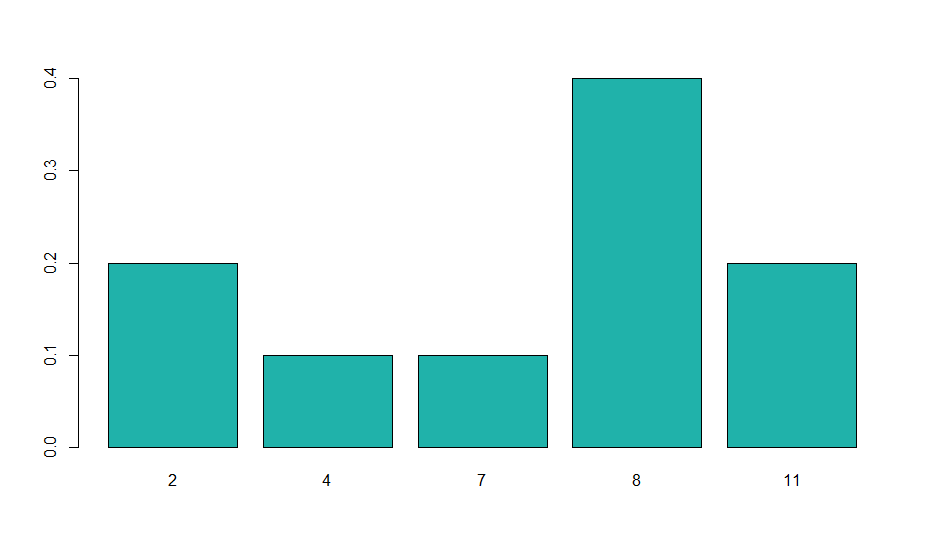
\includegraphics[width=8cm]{../fig/Tut05-20.png}
%\end{center}

Si lo que queremos es ver su función de distribución, podríamos pensar en acumular esas probabilidades:
\begin{knitrout}
\definecolor{shadecolor}{rgb}{0.969, 0.969, 0.969}\color{fgcolor}\begin{kframe}
\begin{alltt}
\hlkwd{barplot}\hlstd{(}\hlkwd{cumsum}\hlstd{(probabilidades),} \hlkwc{names.arg}\hlstd{=valores,} \hlkwc{col}\hlstd{=}\hlstr{"lightseagreen"}\hlstd{)}
\end{alltt}
\end{kframe}
\includegraphics[width=\maxwidth]{figure/unnamed-chunk-16-1} 

\end{knitrout}
Pero este gráfico, como ves,  tiene muchas limitaciones y no es especialmente informativo. Para representar la función de distribución es más común utilizar {\em gráficos de escalera} como el que aparece en la Figura \ref{curso-cap04:fig:GraficaFuncionDistribucionVariableAleatoriaDiscreta} del libro (página \pageref{curso-cap04:fig:GraficaFuncionDistribucionVariableAleatoriaDiscreta}). En R hay varias maneras de hacerlo, más o menos complicadas. Aquí vamos a limitarnos a incluir, sin demasiadas explicaciones, un fragmento de código que produce ese tipo de gráficos a partir de los vectores de valores y probabilidades. Para mostrar su funcionamiento usamos la misma variable $X$ que venimos utilizando para los anteriores gráficos. Si deseas usar el código con otra variable sólo tienes que descomentar y cambiar las dos primeras líneas, en las que se definen los valores y probabilidades. El resto no necesita modificación. A medida que aprendamos más sobre R, este código quedará más claro.

\begin{knitrout}
\definecolor{shadecolor}{rgb}{0.969, 0.969, 0.969}\color{fgcolor}\begin{kframe}
\begin{alltt}
\hlcom{# valoresX = 2:12}
\hlcom{# probabilidadesX = c(1:6,5:1) / 36}

\hlcom{##  NO MODIFIQUES EL RESTO DEL CODIGO ##}

\hlstd{graficoEscalera} \hlkwb{=} \hlkwa{function}\hlstd{(}\hlkwc{valores}\hlstd{,} \hlkwc{probabilidades} \hlstd{)\{}
  \hlstd{probabilidades} \hlkwb{=} \hlstd{probabilidades}\hlopt{/}\hlkwd{sum}\hlstd{(probabilidades)}
  \hlstd{y0} \hlkwb{=} \hlkwd{c}\hlstd{(}\hlnum{0}\hlstd{,}\hlkwd{cumsum}\hlstd{(probabilidades),} \hlnum{1}\hlstd{)}
  \hlstd{x0} \hlkwb{=} \hlkwd{c}\hlstd{(}\hlkwd{min}\hlstd{(valores)}\hlopt{-}\hlnum{1}\hlstd{,valores,} \hlkwd{max}\hlstd{(valores)}\hlopt{+}\hlnum{1}\hlstd{)}
  \hlstd{xA} \hlkwb{=} \hlstd{x0[}\hlopt{-}\hlkwd{length}\hlstd{(x0)]}
  \hlstd{xB} \hlkwb{=} \hlstd{x0[}\hlopt{-}\hlnum{1}\hlstd{]}
  \hlstd{yA} \hlkwb{=} \hlstd{y0[}\hlopt{-}\hlkwd{length}\hlstd{(y0)]}
  \hlkwd{plot}\hlstd{(x0, y0,} \hlkwc{type}\hlstd{=}\hlstr{"n"}\hlstd{,} \hlkwc{xlab}\hlstd{=}\hlstr{"valores"}\hlstd{,} \hlkwc{ylab}\hlstd{=}\hlstr{"probabilidades"}\hlstd{,} \hlkwc{las}\hlstd{=}\hlnum{3}\hlstd{,} \hlkwc{xaxt}\hlstd{=}\hlstr{"n"}\hlstd{)}
  \hlkwd{segments}\hlstd{(xA,yA,xB,yA,} \hlkwc{lwd}\hlstd{=}\hlnum{4}\hlstd{,} \hlkwc{col}\hlstd{=}\hlstr{"red"}\hlstd{)}
  \hlkwd{points}\hlstd{(xA, yA,} \hlkwc{pch}\hlstd{=}\hlnum{16}\hlstd{,} \hlkwc{col}\hlstd{=}\hlstr{"red"}\hlstd{,} \hlkwc{cex}\hlstd{=}\hlnum{1.5}\hlstd{)}
  \hlkwd{axis}\hlstd{(}\hlnum{1}\hlstd{,} \hlkwc{at}\hlstd{=xA,}   \hlkwc{labels}\hlstd{=xA)}
  \hlkwd{segments}\hlstd{(valores, yA[}\hlopt{-}\hlkwd{length}\hlstd{(yA)] , valores, yA[}\hlopt{-}\hlnum{1}\hlstd{],} \hlkwc{lty}\hlstd{=}\hlnum{2}\hlstd{,} \hlkwc{col}\hlstd{=}\hlstr{"blue"}\hlstd{,} \hlkwc{lwd}\hlstd{=}\hlnum{4}\hlstd{)}
\hlstd{\}}
\hlkwd{graficoEscalera}\hlstd{(valoresX, probabilidadesX)}
\end{alltt}
\end{kframe}
\includegraphics[width=\maxwidth]{figure/unnamed-chunk-17-1} 

\end{knitrout}
El resultado, como ves, es bastante más satisfactorio.

\subsection{Un fichero de comandos R para estudiar una variable discreta.}
\label{tut04:subsec:FicheroComandosRParaVaraiableDiscreta}

Al igual que hicimos en el Tutorial02, en el que incluimos un fichero que resumía muchos comandos de Estadística Descriptiva, vamos a incluir aquí el fichero
\begin{center}
  \fichero{./code/Tut04-AnalisisVariableAleatoriaDiscreta.R}{Tut04-AnalisisVariableAleatoriaDiscreta.R}
\end{center}
que reúne los comandos que hemos ido viendo en este Tutorial para trabajar con una variable aleatoria discreta (con un número finito de valores) definida mediante su tabla de densidad.



\section{Ficheros de datos en R: objetos de tipo {\tt data.frame}.}
\label{tut04:sec:FicherosDatosRObjetosDataFrame}
%\section{Tipos de datos en R. Tablas, matrices, data.frames}
\label{tut04:sec:TablasMatricesDataFrames}

Vamos a aprovechar las próximas secciones de este tutorial para mejorar nuestras habilidades como usuarios de R.
Uno de los objetivos de este curso, en esta vertiente más aplicada de los Tutoriales, es poner al lector en contacto con algunos de los problemas más prácticos que se va a encontrar al trabajar con datos. En particular, en algunas ocasiones,
\begin{itemize}
  \item vamos a trabajar con algunos ficheros de datos {\em muy grandes},
  \item que contendrán muchos datos que no vamos a utilizar directamente, de manera que habrá que {\em seleccionar} una parte de los datos,
  \item esos datos no estarán siempre en el formato más cómodo, o más conveniente, así que habrá que {\em transformarlos}.
\end{itemize}
En el anterior Tutorial03 hemos aprendido el manejo básico de las matrices en R. Las matrices, en comparación con los vectores, mejoran nuestra capacidad de trabajar con conjuntos de datos más complicados. Pero para poder afrontar las situaciones a las que nos referíamos más arriba, todavía debemos aprender a superar algunas dificultades. En primer lugar, no hemos aprendido a leer y escribir las matrices usando ficheros (de tipo {\tt csv}, por ejemplo).  En el Tutorial02 hemos usado las funciones {\tt scan} y {\tt cat} para leer y escribir, respectivamente, vectores usando ficheros {\tt csv}. En este tutorial vamos a aprender a usar las dos funciones de R que se emplean más a menudo para leer ficheros de datos, y que son {\tt write.table} y {\tt read.table}.

Aparte de este problema de lectura/escritura de datos, tenemos que aprender a trabajar en R con conjuntos de datos heterogéneos. Para entender a qué nos referimos con esto, vamos a volver a pensar en el fichero
\begin{center}
\fichero{../datos/Tut01-PracticaConCalc.csv}{Tut01-PracticaConCalc.csv},
\end{center}
que utilizamos en el Tutorial01, y que incluía un {\sf conjunto de datos} con tres columnas con 1300 valores de cada una de las variables {\tt var1}, {\tt var2} y {\tt var3}. En la siguiente figura se muestra el comienzo de aquel fichero, abierto con un editor de texto.
    \begin{figure}[h!]	
    \begin{center}
	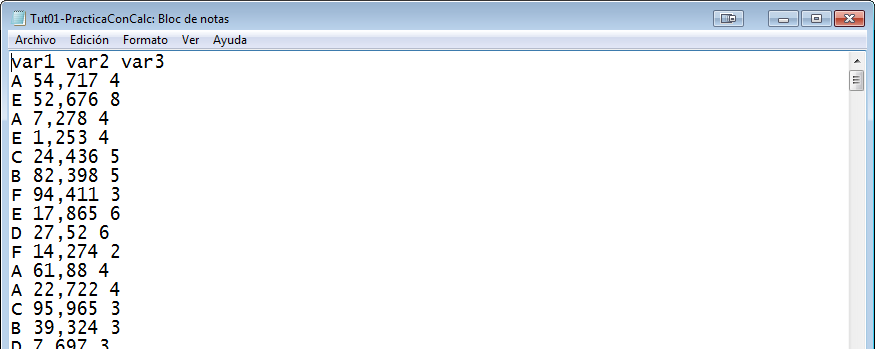
\includegraphics[width=12cm]{../fig/Tut04-08.png}
    \end{center}
	\caption{Contenido del fichero {\tt Tut01-PracticaConCalc.csv}}
    \label{Cap03:fig:FicheroTut01-PracticaConCalc}
    \end{figure}
Lo más importante es observar que las variables que ocupan las columnas de esa tabla son cada una de un tipo distinto: {\tt var1} es una variable de tipo {\tt character} (en el lenguaje de tipos de datos de R; nosotros diríamos que es un factor), {\tt var2} es de tipo {\tt numeric} (una variable cuantitativa continua) y, finalmente, {\tt var3} es de tipo {\tt integer} (una variable cuantitativa discreta). Y además, {\bf esto es esencial}, no queremos separar las columnas para trabajar con ellas por separado, porque los valores de cada fila están relacionados entre sí. Muy a menudo, por ejemplo, cada fila corresponde a una misma observación en la que, para un individuo dado de la población, se han observado los valores de varias variables en ese individuo (por ejemplo, para una misma persona hemos medido su presión arterial, su edad, su peso, etc.)

Para trabajar con este tipo de conjuntos de datos R nos ofrece un tipo de objetos, llamado {\tt data.frame}. A riesgo de ser pesados, la diferencia básica entre una matriz y un {\tt data.frame} es esta:
%
%Hasta ahora, en R, hemos estado trabajando con vectores que, como mucho, servirían para alojar una columna de esta tabla. El único objeto de tipo tabular que hemos usado son las tablas de frecuencia, pero evidentemente necesitamos aprender más sobre el manejo de estructuras de datos más complicadas que los vectores.
%
%En R hay varios tipos, o hablando más propiamente, {\sf estructuras de datos}, adecuadas para trabajar con datos tabulares. La estructura adecuada depende de cómo sea la tabla que vamos a guardar en ellos. Las que más vamos a usar en este curso son:
%\begin{itemize}
%  \item Las que R llama de tipo {\tt table}, como las tablas de frecuencias.
%  \item Las matrices, de tipo {\tt matrix}, con propiedades parecidas a las de las matrices matemáticas. Los {\tt arrays} son como las matrices, pero con más dimensiones: la matriz tiene dos dimensiones (fila y columna), mientras que un {\tt array} puede tener un número cualquiera de dimensiones.
%  \item Los conjuntos de datos, que R llama {\tt data.frames}. A continuación, vamos a explicar por qué son necesarios estos últimos.
%\end{itemize}
%
%Todo nuestro trabajo con R, hasta ahora, se ha centrado en números, que eran valores de variables cuantitativas. Pero sabemos, y nos lo recuerda la variable {\tt var1} del fichero, que a veces es necesario trabajar con variables cualitativas. Es cierto que siempre podríamos codificarlas mediante números.  Pero no es menos cierto que eso sería una limitación, y que lo más conveniente es poder utilizar palabras o frases como valores de las variables. Para hacer esto posible, R nos permite crear un cierto tipo de valores, que  son simplemente palabras o frases entrecomilladas (con comillas dobles; podemos usar las simples).  En general las llamamos {\sf cadenas de texto}, aunque R las identifica como tipo {\tt character}. Por ejemplo, así creamos un vector de valores de una variable cualitativa:
%\begin{verbatim}
%    nombres = c("Io", "Europa", "Ganimedes", "Calisto" )
%\end{verbatim}
%Hasta ahora no hemos sentido la necesidad de preguntarle a R de qué tipo eran los datos que estábamos manejando. Pero ahora, al entrar en escena las variables cualitativas, vamos a aprender a hacerlo. Para ello, abre una nueva sesión en RStudio. Después de guardar todos los ficheros que desees conservar, puedes, por ejemplo, ir al menú {\tt Session} y pulsar en {\tt Clear Workspace}. Contesta afirmativamente a la pregunta que aparece, y será como si R hubiera olvidado las variables con las que hemos estado trabajando antes.
%Verás que la respuesta a
%\begin{center}
%{\tt class(nombres)}
%\end{center}
%es \verb#"character"#, mientras que la respuesta a
%\begin{center}
%{\tt class(diametrosKm)}
%\end{center}
%es \verb#"numeric"#. Todos los vectores con los que hemos trabajado, hasta esta sección, han sido de tipo {\tt numeric}. Aparte de estos dos, hay muchos otros tipos: el tipo {\tt logical}, que sólo toma dos valores, {\tt TRUE} y {\tt FALSE}, y que ya hemos usado en algunas funciones de R (recuerda {\tt sample} con o sin remplazamiento, por ejemplo). Y ahora mismo estamos introduciendo muchos otros tipos nuevos: {\tt table, matrix, array, data.frame}. La lista está lejos de estar acabada, pero para este curso sólo necesitaremos unos pocos tipos más (entre otros, los tipos {\tt factor} y {\tt list}).
%
%Volviendo a este último, el {\tt data.frame}, la justificación de su existencia es precisamente el hecho de que existen varios tipos de datos. Para ser precisos:
%
una matriz (tipo {\tt matrix}) contiene datos en filas y columnas, pero {\em todos del mismo tipo}: todos {\tt numeric} o todos {\tt character}, pero no se admiten mezclas. Y en cambio el {\tt data.frame} permite mezclar datos de distintos tipos.

La ``limitación'', en el caso del {\tt data.frame}, es que los datos de una misma {\em columna} tienen que ser todos del mismo tipo. Pero eso sólo es una limitación a medias, porque, de hecho, vamos a insistir varias veces a lo largo del curso en que esa es la forma adecuada de organizar nuestros datos: cada columna corresponde a una variable, y por lo tanto sus valores son todos de un mismo tipo, el de esa variable (cada fila, por su parte, corresponde a una observación de todas esas variables en un individuo de la población).

\subsection{Operaciones con {\tt data.frames}.}
\label{tut04:subsec:OperacionesConDataFrames}

\subsubsection{Creando un {\tt data.frame} a partir de vectores.}
\label{tut04:subsubsec:CreandoDataFrameVectores}

Podemos crear un {\tt data.frame} a partir de unos cuantos vectores que, eso sí, deben ser de la misma longitud. Cada  uno de los vectores corresponderá a una columna del {\tt data.frame}. Para crear nuestro primer ejemplo de {\tt data.frame}, empieza por ejecutar estos comandos:
\begin{knitrout}
\definecolor{shadecolor}{rgb}{0.969, 0.969, 0.969}\color{fgcolor}\begin{kframe}
\begin{alltt}
    \hlstd{nombres} \hlkwb{=} \hlkwd{c}\hlstd{(}\hlstr{"Io"}\hlstd{,} \hlstr{"Europa"}\hlstd{,} \hlstr{"Ganimedes"}\hlstd{,} \hlstr{"Calisto"} \hlstd{)}
    \hlkwd{class}\hlstd{(nombres)}
\end{alltt}
\begin{verbatim}
## [1] "character"
\end{verbatim}
\begin{alltt}
    \hlstd{diametrosKm} \hlkwb{=} \hlkwd{c}\hlstd{(}\hlnum{3643}\hlstd{,} \hlnum{3122}\hlstd{,} \hlnum{5262}\hlstd{,} \hlnum{4821}\hlstd{)}
    \hlkwd{class}\hlstd{(diametrosKm)}
\end{alltt}
\begin{verbatim}
## [1] "numeric"
\end{verbatim}
\end{kframe}
\end{knitrout}
Para más información, ver el enlace \link{http://es.wikipedia.org/wiki/Sat\%C3\%A9lite\_galileano}{http://es.wikipedia.org/wiki/Satélite\_galileano}.

Hemos usado la función {\tt class} para enfatizar de nuevo el hecho de que los vectores corresponden a tipos distintos de datos. Ahora podemos crear el {\tt data.frame} a partir de esos dos vectores (con los paréntesis exteriores mostraremos la respuesta; R normalmente no lo haría, como sabes):
\begin{knitrout}
\definecolor{shadecolor}{rgb}{0.969, 0.969, 0.969}\color{fgcolor}\begin{kframe}
\begin{alltt}
\hlstd{(satelitesGalileanos} \hlkwb{=} \hlkwd{data.frame}\hlstd{(nombres, diametrosKm) )}
\end{alltt}
\begin{verbatim}
##     nombres diametrosKm
## 1        Io        3643
## 2    Europa        3122
## 3 Ganimedes        5262
## 4   Calisto        4821
\end{verbatim}
\end{kframe}
\end{knitrout}
La respuesta que muestra R nos recuerda (y es, a la vez, distinta) a la que obtenemos al trabajar con una matriz. Los dos tipos de objetos son tabulares, y buena parte de los trucos que hemos aprendido para matrices se aplican también a los {\tt data.frame}. Por ejemplo, vamos a añadir a nuestros datos una columna adicional con el periodo orbital (en días) de cada uno de los satélites galileanos de Jupiter. Esos  datos están almacenados en el vector:
\begin{knitrout}
\definecolor{shadecolor}{rgb}{0.969, 0.969, 0.969}\color{fgcolor}\begin{kframe}
\begin{alltt}
\hlstd{periodoOrbital} \hlkwb{=} \hlkwd{c}\hlstd{(}\hlnum{1.77}\hlstd{,} \hlnum{3.55}\hlstd{,} \hlnum{7.16}\hlstd{,} \hlnum{16.69}\hlstd{)}
\end{alltt}
\end{kframe}
\end{knitrout}
Y para añadirlos como columna al {\tt data.frame} podemos recurrir a la función {\tt cbind} que ya conocemos de las matrices:
\begin{knitrout}
\definecolor{shadecolor}{rgb}{0.969, 0.969, 0.969}\color{fgcolor}\begin{kframe}
\begin{alltt}
\hlstd{(satelitesGalileanos} \hlkwb{=} \hlkwd{cbind}\hlstd{(satelitesGalileanos, periodoOrbital) )}
\end{alltt}
\begin{verbatim}
##     nombres diametrosKm periodoOrbital
## 1        Io        3643           1.77
## 2    Europa        3122           3.55
## 3 Ganimedes        5262           7.16
## 4   Calisto        4821          16.69
\end{verbatim}
\end{kframe}
\end{knitrout}
La notación de corchetes, que usamos con vectores y matrices, también sirve en este caso. Algunos  ejemplos:
\begin{knitrout}
\definecolor{shadecolor}{rgb}{0.969, 0.969, 0.969}\color{fgcolor}\begin{kframe}
\begin{alltt}
\hlstd{satelitesGalileanos[}\hlnum{3}\hlstd{,}\hlnum{2}\hlstd{]}
\end{alltt}
\begin{verbatim}
## [1] 5262
\end{verbatim}
\begin{alltt}
\hlstd{satelitesGalileanos[}\hlnum{1}\hlstd{, ]}
\end{alltt}
\begin{verbatim}
##   nombres diametrosKm periodoOrbital
## 1      Io        3643           1.77
\end{verbatim}
\begin{alltt}
\hlstd{satelitesGalileanos[}\hlkwd{c}\hlstd{(}\hlnum{1}\hlstd{,}\hlnum{4}\hlstd{),} \hlkwd{c}\hlstd{(}\hlnum{1}\hlstd{,}\hlnum{3}\hlstd{)]}
\end{alltt}
\begin{verbatim}
##   nombres periodoOrbital
## 1      Io           1.77
## 4 Calisto          16.69
\end{verbatim}
\end{kframe}
\end{knitrout}
Asegúrate antes de seguir de que has entendido por qué se obtiene esa respuesta en cada uno de los ejemplos. Fíjate, además, en que hemos usado el mismo nombre para el {\tt data.frame} modificado al añadir esa columna.
%\begin{ejercicio}
%\label{tut04:ejercicio04}
%\quad\\
%El satélite {\em Metis} de Júpiter (descubierto en 1979\footnote{Ver \link{http://es.wikipedia.org/wiki/Sat\%C3\%A9lites\_de\_J\%C3\%BApiter}{http://es.wikipedia.org/wiki/Satélites\_de\_Júpiter}}) tiene un diámetro de 43km y un periodo orbital de $0.295$ días. Usa la función {\tt rbind} para añadir los datos de este satélite como última fila del {\tt data.frame}, y guarda el resultado en un {\tt data.frame} llamado {\tt satelitesJupiter}. Solución en la página \pageref{tut04:ejercicio04:sol}.
%\qed
%\end{ejercicio}
También es posible seleccionar elementos del {\tt data.frame} mediante condiciones. Por ejemplo, imagínate que queremos seleccionar los satélites galileanos cuyo diámetro supera los $4000$ kilómetros. Podmeos hacerlo así:
\begin{knitrout}
\definecolor{shadecolor}{rgb}{0.969, 0.969, 0.969}\color{fgcolor}\begin{kframe}
\begin{alltt}
\hlstd{satelitesGalileanos[ (satelitesGalileanos[ ,}\hlnum{2}\hlstd{]} \hlopt{>} \hlnum{4000}\hlstd{) , ]}
\end{alltt}
\begin{verbatim}
##     nombres diametrosKm periodoOrbital
## 3 Ganimedes        5262           7.16
## 4   Calisto        4821          16.69
\end{verbatim}
\end{kframe}
\end{knitrout}
Hemos rodeado con paréntesis la condición para ayudarte a ver la estructura de este comando. Lo que estamos haciendo se puede traducir a palabras así: ``muéstrame las filas de {\tt satelitesGalileanos} tales que la segunda columna sea mayor que 4000''. Y para asegurarnos de que entiendes esa condición entre paréntesis vamos a analizarla con un poco más de detalle.

\begin{ejercicio}
\label{tut04:ejercicio04}
\quad\\
Ejecuta la parte del anterior comando que define la condición,
\begin{knitrout}
\definecolor{shadecolor}{rgb}{0.969, 0.969, 0.969}\color{fgcolor}\begin{kframe}
\begin{alltt}
\hlstd{(satelitesGalileanos[ ,}\hlnum{2}\hlstd{]} \hlopt{>} \hlnum{4000}\hlstd{)}
\end{alltt}
\end{kframe}
\end{knitrout}
e interpreta el resultado. Solución en la página \pageref{tut04:ejercicio04:sol}.
\qed
\end{ejercicio}



\subsubsection{Funciones {\tt read.table} y {\tt write.table}.}
\label{tut04:subsubsec:FuncionesReadWriteTable}


Esta forma de crear un {\tt data.frame}, a partir de vectores, no resuelve nuestro problema inicial de esta sección, el de leer los datos del fichero {\tt Tut01-PracticaConCalc.csv}. Ahora ya sabemos que, una vez leídos, los almacenaremos en un {\tt data.frame}, pero ¿cómo conseguimos que pasen del fichero a ese {\tt data.frame}? Pues usando (entre otras posibilidades) la función {\tt read.table}. Para verla en acción, asegúrate de que has seleccionado como directorio de trabajo (recuerda, menú {\tt Session} de RStudio) la carpeta que contiene el fichero {\tt Tut01-PracticaConCalc.csv}, y ejecuta estos comandos, que explicaremos detenidamente a continuación:
{\small
\begin{knitrout}
\definecolor{shadecolor}{rgb}{0.969, 0.969, 0.969}\color{fgcolor}\begin{kframe}
\begin{alltt}
\hlstd{datosTutorial01} \hlkwb{=}
    \hlkwd{read.table}\hlstd{(}\hlkwc{file}\hlstd{=}\hlstr{"../datos/Tut01-PracticaConCalc.csv"}\hlstd{,} \hlkwc{header}\hlstd{=}\hlnum{TRUE}\hlstd{,} \hlkwc{sep}\hlstd{=}\hlstr{" "}\hlstd{,} \hlkwc{dec}\hlstd{=}\hlstr{","}\hlstd{)}
\hlkwd{class}\hlstd{(datosTutorial01)}
\end{alltt}
\begin{verbatim}
## [1] "data.frame"
\end{verbatim}
\begin{alltt}
\hlkwd{head}\hlstd{(datosTutorial01)}
\end{alltt}
\begin{verbatim}
##   var1  var2 var3
## 1    A 54.72    4
## 2    E 52.68    8
## 3    A  7.28    4
## 4    E  1.25    4
## 5    C 24.44    5
## 6    B 82.40    5
\end{verbatim}
\end{kframe}
\end{knitrout}
}
La función {\tt read.table} se encarga de leer el fichero {\tt csv} y guardar su contenido en un {\tt data.frame}. Enseguida volvemos sobre los argumentos de {\tt read.table}.Pero antes, fíjate en que el resultado de {\tt class} muestra que {\tt datosTutorial01} es, de hecho, un {data.frame}. Hemos visto anteriormente que el comando {\tt head}  se puede usar para mostrar el comienzo de un vector, mientras que  {\tt tail} muestra el final. Ambos comandos se pueden usar igualmente con {\tt data.frames}, para obtener, respectivamente, las primeras o últimas filas del {\tt data.frame} (que tiene 1300 filas).

Veamos ahora los argumentos de {\tt read.table}:
\begin{itemize}
  \item El primero, {\tt file}, apenas necesita explicación. Asegúrate, eso sí, de que el fichero que vas a usar está en tu directorio de trabajo. Si es así, tras escribir {\tt file=""} en RStudio basta con que pulses el tabulador para ahorrarte errores y trabajo.
  \item La opción {\tt header} nos permite decirle a R si el fichero {\tt csv} incluye una primera fila en la que aparecen los nombres de las variables (usamos {\tt TRUE} en este caso) o no (y usamos {\tt FALSE}). Si el fichero no incluye esa línea, R pondrá nombres a las variables por nosotros, de forma automática, y no siempre nos gustará el resultado (aunque siempre podemos ponerlos sobre la marcha con la opción {\tt col.names}).
  \item La opción {\tt sep} le dice a R como están separados (con comas, espacios, etc.) los valores de las distintas variables, dentro de cada fila del fichero {\tt csv}.
  \item Finalmente (para este ejemplo), la opción {\tt dec} nos permite indicarle a R si se usan puntos o comas para separar los decimales. El programa R siempre trabajará, en sus operaciones internas, con el punto como separador, pero gracias a esta opción resulta fácil leer ficheros de datos en el formato (desgraciadamente, todavía) habitual en España y otros países.
\end{itemize}

En resumen, ya hemos leído el fichero {\tt csv} llamado {\tt Tut01-PracticaConCalc.csv}, lo hemos guardado en un {\tt data.frame} llamado {\tt datosTutorial01}, y seguramente, podemos ponernos a hacer cosas con las variables {\tt var1, var2, var3} que corresponden a las columnas de ese fichero. Vamos a tratar de calcular, por ejemplo, la media de {\tt var3}:
\begin{knitrout}
\definecolor{shadecolor}{rgb}{0.969, 0.969, 0.969}\color{fgcolor}\begin{kframe}
\begin{alltt}
\hlkwd{mean}\hlstd{(var3)}
\end{alltt}


{\ttfamily\noindent\bfseries\color{errorcolor}{\#\# Error in mean(var3): object 'var3' not found}}\end{kframe}
\end{knitrout}
La respuesta de R, en color rojo, indica que se ha enfadado con nosotros. ¿Por qué? Pues porque las variables de un {\tt data.frame} no viven vidas propias. El nombre correcto de esta variable no es {\tt var3} sino   \verb#datosTutorial01$var3#.

Y lo mismo sucede con {\tt var1} y {\tt var2}, claro. Si pruebas con ese nombre, el cálculo de la media funcionará sin problemas:
\begin{knitrout}
\definecolor{shadecolor}{rgb}{0.969, 0.969, 0.969}\color{fgcolor}\begin{kframe}
\begin{alltt}
\hlkwd{mean}\hlstd{(datosTutorial01}\hlopt{$}\hlstd{var3)}
\end{alltt}
\begin{verbatim}
## [1] 5.04
\end{verbatim}
\end{kframe}
\end{knitrout}
``Entonces, cada vez que quiera referirme a esta variable, ¿tengo que escribir {\tt datosTutorial01\$var3}?'' La respuesta corta es: sí. La respuesta larga es que,
\begin{itemize}
  \item[(a)] por un lado, así evitamos confusiones entre variables con el mismo nombre, pero procedentes de distintos {\tt data.frames},
  \item[(b)] usando el tabulador en RStudio, este problema se alivia mucho. Tras escribir sólo las tres letras {\tt dat}, si pulso el tabulador aparece el nombre del {\tt data.frame}. Y si acepto ese nombre, y a continuación escribo {\tt\$} (de manera que tengo escrito {\tt datosTutorial01\$}), entonces una nueva pulsación del tabulador me permite acceder a la variable que deseo, fácilmente y sin errores.
  \item[(c)] existen funciones (como {\tt attach} o {\tt with}) que nos permite aliviar este problema, {\em cuando sabemos bien lo que hacemos}. Más adelante veremos  algunos ejemplos.
\end{itemize}


Antes de seguir adelante, vamos a pensar un momento en el proceso contrario, en el que tenemos un {\tt data.frame} y queremos escribirlo en un fichero {\tt csv}. La función correspondiente se llama, como era de esperar, {\tt write.table}, y vamos a explorar su funcionamiento mediante algunos ejercicios.

\begin{ejercicio}
\label{tut04:ejercicio05}
\quad\\
\begin{enumerate}
  \item Vamos a fabricar un {\tt data.frame}, con $300$ filas y $3$ columnas, usando tres vectores. El primero será un vector con las letras {\tt A}, {\tt B} y {\tt C}, repetidas cada una $100$ veces. Concretamente, las posiciones de la $1$ a la $100$ serán {\tt A}, las $100$ siguientes {\tt B} y las $100$ últimas {\tt C}. El segundo vector estará formado por $300$ números enteros, elegidos al azar entre $-100$ y $100$ (usa {\tt set.seed(2014)} para poder comparar tus soluciones con las nuestras). Para fabricar el tercer vector usa el comando {\tt rnorm(300)}. Pronto aprenderemos su significado, pero te podemos adelantar que genera números reales al azar (pero no todos los valores son igual de probables). Cuando tengas los tres vectores úsalos para crear un {\tt data.frame} llamado {\tt Tut04WriteTable}, y comprueba su contenido con las funciones {\tt head} y {\tt tail}.\\
\begin{knitrout}
\definecolor{shadecolor}{rgb}{0.969, 0.969, 0.969}\color{fgcolor}\begin{kframe}
\begin{verbatim}
##   vector1 vector2 vector3
## 1       A     -43 -0.0557
## 2       A     -67  0.7253
## 3       A      25  1.0051
## 4       A     -38  0.1155
## 5       A      10  0.2637
## 6       A     -83  0.9814
##     vector1 vector2 vector3
## 295       C      81   1.126
## 296       C     -67   0.383
## 297       C      38  -0.645
## 298       C     -71  -0.805
## 299       C      -1  -0.703
## 300       C      89   1.841
\end{verbatim}
\end{kframe}
\end{knitrout}
  \item Para guardar el {\tt data.frame} en un fichero, llamado {\tt Tut04WriteTable.csv}, asegúrate de que sabes cual es el directorio de trabajo (ejecuta {\tt getwd()} si dudas), y usa la función {\tt write.table} así:
\begin{knitrout}
\definecolor{shadecolor}{rgb}{0.969, 0.969, 0.969}\color{fgcolor}\begin{kframe}
\begin{alltt}
  \hlkwd{write.table}\hlstd{(Tut04WriteTable,} \hlkwc{file}\hlstd{=}\hlstr{"../datos/Tut04WriteTable.csv"}\hlstd{)}
\end{alltt}
\end{kframe}
\end{knitrout}
      Después comprueba, usando un editor de texto (como el Bloc de Notas), que el contenido del fichero es correcto.
  \item Abre el fichero {\tt csv} que has creado con Calc, como aprendimos a hacer en el Tutorial00 (usa un espacio como separador), y calcula, con Calc,  la media de la tercera columna de la tabla (el {\tt vector3} que hemos creado en R). ¿Qué dificultades te encuentras?
  \item Para soslayar esas dificultades vamos a ejecutar otra versión de la función {\tt write.table}, que dará ocmo resultado un nuevo fichero {\tt csv} (hemos añadido un {\tt 2} al nombre del fichero, para distinguirlos).
      {\small
\begin{knitrout}
\definecolor{shadecolor}{rgb}{0.969, 0.969, 0.969}\color{fgcolor}\begin{kframe}
\begin{alltt}
\hlkwd{write.table}\hlstd{(Tut04WriteTable,} \hlkwc{file}\hlstd{=}\hlstr{"../datos/Tut04WriteTable2.csv"}\hlstd{,} \hlkwc{dec} \hlstd{=} \hlstr{","}\hlstd{,} \hlkwc{row.names} \hlstd{=} \hlnum{FALSE}\hlstd{)}
\end{alltt}
\end{kframe}
\end{knitrout}
      }
      Abre este nuevo fichero con Calc, y completa la tarea pendiente del apartado anterior. Comprueba con R el valor de la media.

\end{enumerate}
Solución en la página \pageref{tut04:ejercicio05:sol}.
\qed
\end{ejercicio}

\subsection{Funciones para trabajar con {\tt data.frames}.}

El punto de partida de casi todo el trabajo que se hace en R es, a menudo, un {\tt data.frame} (o algún tipo de objeto similar). Ese {\tt data.frame} puede ser el resultado de leer un fichero con {\tt read.table}. Otra posibilidad, que no vamos a explorar por el momento, es la de usar funciones de R para descargar los datos directamente desde internet, y guardar esos datos descargados en un {\tt data.frame}. En una sesión típica de trabajo, una vez que tenemos un conjunto (o conjuntos) de datos almacenados en un {\tt data.frame} (o en varios), a continuación realizamos algún tipo de análisis, más o menos complicado con esos datos, y guardamos el resultado en un nuevo {\tt data.frame}, que a su vez puede exportarse a algún fichero (por ejemplo, guardando el resultado en un fichero {\tt csv}). Conviene tener en cuenta, no obstante, que si guardamos los datos de partida y el fichero de comandos de R que hemos usado (¡bien comentado!), nuestro trabajo será, en gran medida, reproducible.  Ya veremos algún ejemplo más detallado, más adelante en el curso.

Por el momento, lo que queremos transmitirle al lector es que aprender a manejar los {\tt data.frame} de R, al menos de forma básica, es un requisito imprescindible para utilizar el programa de forma eficaz. Y por esa razón vamos a aprender algunas funciones adicionales, que hacen más cómodo nuestro trabajo con los {\tt data.frames}.

Para empezar, las funciones {\tt nrow} y {\tt ncol} nos permiten obtener el número de filas y columnas de un {\tt data.frame}.
\begin{knitrout}
\definecolor{shadecolor}{rgb}{0.969, 0.969, 0.969}\color{fgcolor}\begin{kframe}
\begin{alltt}
\hlkwd{nrow}\hlstd{(satelitesGalileanos)}
\end{alltt}
\begin{verbatim}
## [1] 4
\end{verbatim}
\begin{alltt}
\hlkwd{ncol}\hlstd{(satelitesGalileanos)}
\end{alltt}
\begin{verbatim}
## [1] 3
\end{verbatim}
\end{kframe}
\end{knitrout}
En un {\tt data.frame} tan pequeño esto puede parecer trivial, pero cuando trabajemos con miles de filas, y cientos de columnas, se hará inevitable.

Otra función útil es la función {\tt colnames} que nos permite obtener, pero también modificar, los nombres de las columnas.
\begin{knitrout}
\definecolor{shadecolor}{rgb}{0.969, 0.969, 0.969}\color{fgcolor}\begin{kframe}
\begin{alltt}
\hlkwd{colnames}\hlstd{(satelitesGalileanos)}
\end{alltt}
\begin{verbatim}
## [1] "nombres"        "diametrosKm"    "periodoOrbital"
\end{verbatim}
\end{kframe}
\end{knitrout}
Fijate en el resultado de este comando, que mostramos usando {\tt head}:
\begin{knitrout}
\definecolor{shadecolor}{rgb}{0.969, 0.969, 0.969}\color{fgcolor}\begin{kframe}
\begin{alltt}
\hlkwd{colnames}\hlstd{(satelitesGalileanos)} \hlkwb{=} \hlkwd{c}\hlstd{(}\hlstr{"varUno"}\hlstd{,} \hlstr{"varDos"}\hlstd{,} \hlstr{"varTres"}\hlstd{)}
\hlkwd{head}\hlstd{(satelitesGalileanos)}
\end{alltt}
\begin{verbatim}
##      varUno varDos varTres
## 1        Io   3643    1.77
## 2    Europa   3122    3.55
## 3 Ganimedes   5262    7.16
## 4   Calisto   4821   16.69
\end{verbatim}
\end{kframe}
\end{knitrout}

\begin{ejercicio}
\label{tut04:ejercicio06}
\quad\\
\begin{enumerate}
  \item Devuelve el {\tt data.frame} a su estado anterior, y comprueba el resultado con {\tt head}.
  \item ¿Qué resultado se obtiene al aplicar la función {\tt dim} al {\tt data.frame}?
\end{enumerate}
Soluciones en la página \pageref{tut04:ejercicio06:sol}.
\qed
\end{ejercicio}

La función {\tt str} (puedes pensar que es una abreviatura de {\em structure}) es una función cuyo uso no se limita a los {\tt data.frame}, y que nos proporciona información útil sobre los componentes del objeto de interés. Un par de ejemplos:
\begin{knitrout}
\definecolor{shadecolor}{rgb}{0.969, 0.969, 0.969}\color{fgcolor}\begin{kframe}
\begin{alltt}
\hlkwd{str}\hlstd{(satelitesGalileanos)}
\end{alltt}
\begin{verbatim}
## 'data.frame':	4 obs. of  3 variables:
##  $ varUno : Factor w/ 4 levels "Calisto","Europa",..: 4 2 3 1
##  $ varDos : num  3643 3122 5262 4821
##  $ varTres: num  1.77 3.55 7.16 16.69
\end{verbatim}
\begin{alltt}
\hlkwd{str}\hlstd{(Tut04WriteTable)}
\end{alltt}
\begin{verbatim}
## 'data.frame':	300 obs. of  3 variables:
##  $ vector1: Factor w/ 3 levels "A","B","C": 1 1 1 1 1 1 1 1 1 1 ...
##  $ vector2: int  -43 -67 25 -38 10 -83 83 20 -81 -69 ...
##  $ vector3: num  -0.0557 0.7253 1.0051 0.1155 0.2637 ...
\end{verbatim}
\end{kframe}
\end{knitrout}
Como ves, el resultado es una descripción del conjunto de datos: qué variables lo forman y de qué tipo son, además del número de observaciones (filas) del conjunto de datos, y algunos valores iniciales de cada variable.

A lo largo del curso iremos conociendo más funciones que nos facilitarán el trabajo con {\tt data.frames}, con el objetivo de ser capaces de seleccionar y transformar los datos, como decíamos al principio de esta sección.


\subsection{Conversión entre tipos de datos}
\label{tut04:subsec:ConversionTiposDatos}

La función {\tt read.table} siempre produce como resultado un {\tt data.frame}. Y ya sabemos que la razón por la que usamos un {\tt data.frame} es para poder trabajar con tablas, cuyas columnas contienen variables de distintos tipos. Las matrices, en cambio, tienen todas sus columnas del mismo tipo. Pero, puesto que en cualquier caso son también tablas, muchas veces usaremos ficheros {\tt csv} para almacenar matrices, y leeremos esos ficheros usando la función {\tt read.table}.

Por ejemplo, el fichero
\begin{center}
  \fichero{../datos/Tut04-Matriz.csv}{Tut04-Matriz.csv}
\end{center}
contiene una matriz $10\times 10$ de números enteros. La siguiente figura muestra el contenido del fichero, tal y como se ve usando el {\em Bloc de Notas}:



Las distintas estructuras de datos, y la capacidad de R para modificarlas, nos pueden ser de utilidad a la hora de manipular ficheros de datos. Imagínate que tenemos un fichero de datos en el que los datos aparecen en forma de tabla, como el fichero \fichero{../datos/Tut05-DatosEnTabla.csv}{Tut05-DatosEnTabla.csv}, que en la siguiente figura mostramos abierto en el Bloc de Notas de Windows. Los datos, como puede verse, están separados por espacios, pero cada fila contiene 10 datos.
    \begin{center}
    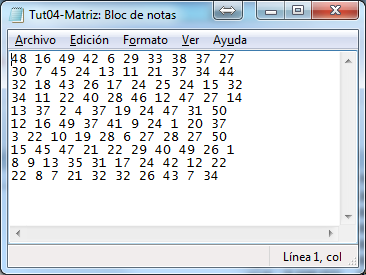
\includegraphics[width=11cm]{../fig/Tut04-21.png}
    \end{center}
Para abrir este fichero con R (fijamos el directorio de trabajo y) usamos el comando
\begin{knitrout}
\definecolor{shadecolor}{rgb}{0.969, 0.969, 0.969}\color{fgcolor}\begin{kframe}
\begin{alltt}
\hlstd{(datos} \hlkwb{=} \hlkwd{read.table}\hlstd{(}\hlkwc{file}\hlstd{=}\hlstr{"../datos/Tut04-Matriz.csv"}\hlstd{,} \hlkwc{sep}\hlstd{=}\hlstr{" "}\hlstd{))}
\end{alltt}
\end{kframe}
\end{knitrout}
\vspace{-6.7mm}
\begin{knitrout}
\definecolor{shadecolor}{rgb}{0.969, 0.969, 0.969}\color{fgcolor}\begin{kframe}
\begin{verbatim}
##    V1 V2 V3 V4 V5 V6 V7 V8 V9 V10
## 1  48 16 49 42  6 29 33 38 37  27
## 2  30  7 45 24 13 11 21 37 34  44
## 3  32 18 43 26 17 24 25 24 15  32
## 4  34 11 22 40 28 46 12 47 27  14
## 5  13 37  2  4 37 19 24 47 31  50
## 6  12 16 49 37 41  9 24  1 20  37
## 7   3 22 10 19 28  6 27 28 27  50
## 8  15 45 47 21 22 29 40 49 26   1
## 9   8  9 13 35 31 17 24 42 12  22
## 10 22  8  7 21 32 32 26 43  7  34
\end{verbatim}
\end{kframe}
\end{knitrout}
\vspace{-0.7cm}
\begin{knitrout}
\definecolor{shadecolor}{rgb}{0.969, 0.969, 0.969}\color{fgcolor}\begin{kframe}
\begin{alltt}
\hlkwd{class}\hlstd{(datos)}
\end{alltt}
\begin{verbatim}
## [1] "data.frame"
\end{verbatim}
\end{kframe}
\end{knitrout}
El resultado de la función {\tt class} demuestra que la variable {\tt datos} es de tipo {\tt data.frame}, porque ese es el resultado que produce siempre {\tt read.table}. De hecho, R piensa que la interpretación natural de este fichero es pensar que se trata de 10 observaciones (una por fila) de 10 variables (una por columna), y por eso ha añadido, de su cosecha, nombres para esas variables, llamándolas {\tt V1, V2,...,V10}.

No es eso lo que queremos, claro. Pero, afortunadamente, R nos ofrece varias funciones que permiten convertir un {\tt data.frame} en una matriz o un vector, si esas conversiones tienen sentido. En este ejemplo usaremos la función {\tt as.matrix}, de este modo:
\begin{knitrout}
\definecolor{shadecolor}{rgb}{0.969, 0.969, 0.969}\color{fgcolor}\begin{kframe}
\begin{alltt}
\hlstd{(matrizDatos} \hlkwb{=} \hlkwd{as.matrix}\hlstd{(datos))}
\end{alltt}
\begin{verbatim}
##       V1 V2 V3 V4 V5 V6 V7 V8 V9 V10
##  [1,] 48 16 49 42  6 29 33 38 37  27
##  [2,] 30  7 45 24 13 11 21 37 34  44
##  [3,] 32 18 43 26 17 24 25 24 15  32
##  [4,] 34 11 22 40 28 46 12 47 27  14
##  [5,] 13 37  2  4 37 19 24 47 31  50
##  [6,] 12 16 49 37 41  9 24  1 20  37
##  [7,]  3 22 10 19 28  6 27 28 27  50
##  [8,] 15 45 47 21 22 29 40 49 26   1
##  [9,]  8  9 13 35 31 17 24 42 12  22
## [10,] 22  8  7 21 32 32 26 43  7  34
\end{verbatim}
\begin{alltt}
\hlkwd{class}\hlstd{(matrizDatos)}
\end{alltt}
\begin{verbatim}
## [1] "matrix"
\end{verbatim}
\end{kframe}
\end{knitrout}
Así que ya tenemos una matriz de R. Fíjate en que el formato de la respuesta (los nombres de filas) para esta matriz es diferente del formato del {\tt data.frame} anterior. Para evitar una posible pérdida de información R ha conservado los nombres de las columnas, pero podemos librarnos de ellos fácilmente.
\begin{knitrout}
\definecolor{shadecolor}{rgb}{0.969, 0.969, 0.969}\color{fgcolor}\begin{kframe}
\begin{alltt}
\hlkwd{colnames}\hlstd{(matrizDatos)} \hlkwb{=} \hlkwa{NULL}
\hlstd{matrizDatos}
\end{alltt}
\begin{verbatim}
##       [,1] [,2] [,3] [,4] [,5] [,6] [,7] [,8] [,9] [,10]
##  [1,]   48   16   49   42    6   29   33   38   37    27
##  [2,]   30    7   45   24   13   11   21   37   34    44
##  [3,]   32   18   43   26   17   24   25   24   15    32
##  [4,]   34   11   22   40   28   46   12   47   27    14
##  [5,]   13   37    2    4   37   19   24   47   31    50
##  [6,]   12   16   49   37   41    9   24    1   20    37
##  [7,]    3   22   10   19   28    6   27   28   27    50
##  [8,]   15   45   47   21   22   29   40   49   26     1
##  [9,]    8    9   13   35   31   17   24   42   12    22
## [10,]   22    8    7   21   32   32   26   43    7    34
\end{verbatim}
\end{kframe}
\end{knitrout}
Ya sabemos que la función {\tt write.table} nos permite guardar un {\tt data.frame} en un fichero {\tt csv} (en realidad, en un fichero de texto; la extensión puede ser {\tt txt}, {\tt .dat}, o la que queramos). Pero también podemos usarla para escribir otros objetos de R, como matrices o vectores (y en ese caso,
sustituye a la función {\tt cat} que vimos en el Tutorial02).

Para que puedas practicar esto, haremos algunos ejercicios.
\begin{ejercicio}
\label{tut04:ejercicio07}
\quad\\
\begin{enumerate}
  \item Construye la matriz traspuesta de {\tt matrizDatos}  y guárdala en un fichero llamado {\tt traspuesta.csv}. No queremos que el fichero contenga nada, excepto los números de la matriz, separados por espacios. Piensa, además, en lo que habrías tenido que hacer para hacer este trabajo a mano, sin usar R.
  \item El fichero
  \begin{center}
  \fichero{../datos/Tut04-3000datos.csv}{Tut04-3000datos.csv}
  \end{center}
  contiene una lista de 3000 números, escritos en forma de tabla de 5 columnas y 600 filas (de nuevo, para evitarte cualquier tentación de hacer el trabajo a mano). El objetivo de este ejercicio es convertir esos datos a un fichero {\tt csv} con una única columna en la que aparezcan esos mismos 3000 números (leyendo por filas la tabla, de manera que la columna resultante empezará con los elementos de la primera fila de la tabla).
\end{enumerate}
Solución en la página \pageref{tut04:ejercicio07:sol}.
\qed
\end{ejercicio}


%##############################################################################################################




%%\textcolor{red}{\Huge AQUÍ ESTOY}
%\pendiente{\LARGE AQUÍ}
%
%\newpage



\section{Condicionales {\tt if-else} y bucles {\tt for} en R.}
%\label{tut05:sec:CondicionalesBucleForR}
\label{tut04:sec:CondicionalesBucleForR}

\noindent{\bf Opcional: esta sección puede omitirse en una primera lectura.}\\

Si R ha llegado a la posición que ahora ocupa, y si su radio de acción no deja de crecer, es sobre todo porque no se limita a ser un programa de Estadística más al uso, con cada vez más opciones en los menús. Ante todo, R es un lenguaje de programación, con un fuerte sesgo -desde luego- hacia el Análisis de Datos y la Estadística. Para sacarle todo el partido a R hay que aprender algo de programación.

Y un programa, en código R, es un conjunto de instrucciones, como los que ya hemos aprendido a escribir, pero que toma decisiones por nosotros de forma automática, y que en función de esas decisiones puede repetir un conjunto de instrucciones una cierta cantidad de veces. Esos dos ingredientes, las decisiones, mediante {\sf condicionales}, y la repetición, mediante {\sf bucles}, son los dos pilares básicos de la programación en R, y en casi cualquier otro lenguaje de programación. En este tutorial vamos a aprender a usar los condicionales, y el tipo de bucle más sencillo, usándolos para ilustrar problemas sobre el Teorema de la Probabilidad Total.

Para empezar, veamos un ejemplo muy sencillo de toma de decisiones. La decisión más básica consiste siempre en elegir entre dos caminos posibles (en general, dos opciones; pero la imagen del camino ayuda a pensar).  Y el esquema de una decisión básica siempre es este:
\begin{center}
\begin{minipage}{12cm}
    {\em Si se cumple {\bf cierta condición}, entonces\\
    \phantom{palabra} vamos por {\bf el camino A}.\\
    Y si no se cumple, \\
    \phantom{palabra} vamos por {\bf el camino B}.}
\end{minipage}
\end{center}
Las frases que hemos destacado, en negrita, son las que cambiarán en cada caso concreto, porque en cada ejemplo la condición será distinta, y distintos serán también los caminos A y B. Pero la forma de la frase es la misma siempre. Para traducir una frase de esta forma al lenguaje de R disponemos de un estructura especial que, esquemáticamente, dejando todavía sin traducir las partes destacadas de la frase, funciona así:
\begin{knitrout}
\definecolor{shadecolor}{rgb}{0.969, 0.969, 0.969}\color{fgcolor}\begin{kframe}
\begin{verbatim}

if(se cumple cierta condicion){
  vamos por el camino A
} else {
  vamos por el camino B
}
\end{verbatim}
\end{kframe}
\end{knitrout}
Veamos un ejemplo de decisión más concreto. Vamos a lanzar un dado (usando la función {\tt sample} de R).  Si el resultado es mayor o igual que  tres, entonces gano un euro. Y si eso no se cumple (es decir, si es menor que tres),  pierdo un euro. Vamos a escribir un fragmento de código R que calcule mis ganancias o pérdidas después de este juego tan sencillo. En R esto se convierte en:
\begin{knitrout}
\definecolor{shadecolor}{rgb}{0.969, 0.969, 0.969}\color{fgcolor}\begin{kframe}
\begin{alltt}
    \hlstd{(dado}\hlkwb{=}\hlkwd{sample}\hlstd{(}\hlnum{1}\hlopt{:}\hlnum{6}\hlstd{,}\hlnum{1}\hlstd{))}

    \hlkwa{if}\hlstd{(dado} \hlopt{>=} \hlnum{3}\hlstd{)\{}
        \hlstd{ganancia} \hlkwb{=} \hlnum{1}
    \hlstd{\}} \hlkwa{else} \hlstd{\{}
        \hlstd{ganancia} \hlkwb{=} \hlopt{-}\hlnum{1}
    \hlstd{\}}

    \hlstd{ganancia}
\end{alltt}
\end{kframe}
\end{knitrout}
Antes de seguir adelante es una buena idea que ejecutes varias veces este código para que veas que, en efecto, se obtienen las respuestas esperadas según sea el resultado del dado.

El primer paso de una estructura condicional {\tt if/else} es, naturalmente, una condición. Las condiciones en R son {\sf expresiones booleanas (o lógicas)}, que ya hemos visto en la Sección \ref{tut02-tut02:subsubsec:SeleccionElementosCondicionesValoresBooleanosWhich}
(pág. \pageref{tut02-tut02:subsubsec:SeleccionElementosCondicionesValoresBooleanosWhich}) del Tutorial02. Es decir, una fórmula que sólo puede tomar dos valores, verdadero o falso.
La fórmula {\tt dado >= 3} es una de estas fórmulas lógicas, porque al sustituir cada valor concreto de {\tt dado}, el resultado será verdadero o falso, dos valores que que en R se representan mediante dos expresiones que ya conocemos, {\tt TRUE} y {\tt FALSE}. Para ver esto con más detalle, vamos a ver un par de ejemplos de ejecución del código de la condición (cuando tú lo ejecutes obtendrás otros resultados, claro):
\begin{knitrout}
\definecolor{shadecolor}{rgb}{0.969, 0.969, 0.969}\color{fgcolor}\begin{kframe}
\begin{alltt}
    \hlstd{(dado} \hlkwb{=} \hlkwd{sample}\hlstd{(}\hlnum{1}\hlopt{:}\hlnum{6}\hlstd{,}\hlnum{1}\hlstd{))}
\end{alltt}
\begin{verbatim}
## [1] 5
\end{verbatim}
\begin{alltt}
    \hlstd{dado} \hlopt{>=} \hlnum{3}
\end{alltt}
\begin{verbatim}
## [1] TRUE
\end{verbatim}
\begin{alltt}
    \hlstd{(dado} \hlkwb{=} \hlkwd{sample}\hlstd{(}\hlnum{1}\hlopt{:}\hlnum{6}\hlstd{,}\hlnum{1}\hlstd{))}
\end{alltt}
\begin{verbatim}
## [1] 1
\end{verbatim}
\begin{alltt}
    \hlstd{dado} \hlopt{>=} \hlnum{3}
\end{alltt}
\begin{verbatim}
## [1] FALSE
\end{verbatim}
\end{kframe}
\end{knitrout}
En este fragmento de código no usamos el resultado de la condición (o fórmula lógica) {\tt dado >= 3} para nada. Nos limitamos a {\em calcular} esa fórmula y mostrar el resultado. Ejecuta estos comandos varias veces. Obtendrás {\tt TRUE} o {\tt FALSE} como resultado según cual haya sido el resultado de {\tt dado}, claro. Si es necesario, vuelve ahora al primer ejemplo de {\tt if else} que hemos visto, y asegúrate de que entiendes su mecanismo.


Las fórmulas booleanas, o lógicas, pueden ser muy sencillas, como ese {\tt dado >= 3} que hemos visto, o pueden ser bastante más complicadas. Iremos aprendiendo más sobre ellas a lo largo del curso, pero podemos adelantarte que están muy relacionadas con las operaciones de unión e intersección que hacemos con los sucesos en Probabilidad. Al fin y al cabo, un suceso $A$ es algo que puede ocurrir o no ocurrir, y eso es similar a decir que $A$ es {\tt TRUE} cuando ocurre, y {\tt FALSE} cuando no ocurre. Y de la misma forma que combinamos los sucesos con:
\begin{itemize}
  \item uniones (A o B),
  \item intersecciones ( A y B)
  \item y complementarios (no A, o lo contrario de A),
\end{itemize}
también aprenderemos a combinar las fórmulas booleanas con operaciones análogas. Pero antes, vamos a ver un ejemplo más elaborado de estructura {\tt if-else}, relacionado con el Teorema de las Probabilidades Totales. Esta es la descripción del problema:

\begin{center}
\begin{minipage}{12cm}
{\em Tiramos un dado. Si el resultado es menor que 5, usamos una urna con 1 bola blanca y 9 negras. Si es 5 o 6, usamos una urna con 4 bolas blancas y 3 bolas negras. En cualquiera de los dos casos, extraemos una bola al azar. ¿Cuál es la probabilidad de que esa bola sea negra?}
\end{minipage}
\end{center}

El Teorema de las Probabilidades Totales proporciona este valor de la probabilidad:
\[P(\mbox{bola negra})=P(\mbox{bola negra}\,|\,\mbox{urna 1})P(\mbox{urna 1})+P(\mbox{bola negra}\,|\,\mbox{urna 2})P(\mbox{urna 2})=\]
\[\dfrac{4}{6}\cdot\dfrac{9}{10}+\dfrac{2}{6}\cdot\dfrac{3}{7}=\dfrac{26}{35}\approx 0.743\]
Y lo que vamos a hacer es usar R para comprobar ``experimentalmente'' este resultado, mediante una simulación, como hemos hecho en otras ocasiones. Para hacer esto necesitamos un fragmento de código R que tire un dado y, en función del resultado del dado, elija una urna y extraiga una bola de esa urna. Para empezar escribimos este esquema del código, que todavía no funciona. Es un {\em borrador} del código definitivo, que de momento sólo contiene la estructura {\tt if/else} básica, acompañada de comentarios que nos dicen lo que queremos hacer al tomar cada uno de los dos caminos (o ramas, o brazos, que de todas esas formas se llaman):
\begin{knitrout}
\definecolor{shadecolor}{rgb}{0.969, 0.969, 0.969}\color{fgcolor}\begin{kframe}
\begin{alltt}
    \hlcom{# Tiramos el dado.}
    \hlstd{(dado} \hlkwb{=} \hlkwd{sample}\hlstd{(}\hlnum{1}\hlopt{:}\hlnum{6}\hlstd{,}\hlnum{1}\hlstd{))}
    \hlcom{# y, según el resultado, elegimos urna.}
    \hlkwa{if}\hlstd{(dado} \hlopt{<} \hlnum{5}\hlstd{)\{}
        \hlcom{# Usamos la urna 1 para elegir la bola.}
    \hlstd{\}} \hlkwa{else} \hlstd{\{}
        \hlcom{# Usamos la urna 2 para elegir la bola.}
    \hlstd{\}}
    \hlcom{# Y, al final, mostraremos la bola que ha salido.}
\end{alltt}
\end{kframe}
\end{knitrout}
Para escribir el código que falta, supongamos por un momento que el dado ha resultado menor que 5. Entonces tenemos que sacar una bola blanca o negra de la urna 1. Como se trata de un sorteo, vamos a usar la función {\tt sample}. Podríamos usar números para codificar los colores blanco y negro, diciendo por ejemplo que 1 es blanco y 2 es negro. Pero vamos a hacer algo mejor, y vamos a aplicar {\tt sample} a un vector de caracteres, así (añadimos paréntesis para que veas el tipo de resultado que se obtiene):
\begin{knitrout}
\definecolor{shadecolor}{rgb}{0.969, 0.969, 0.969}\color{fgcolor}\begin{kframe}
\begin{alltt}
\hlstd{(bolaUrna1} \hlkwb{=} \hlkwd{sample}\hlstd{(} \hlkwd{c}\hlstd{(}\hlstr{"blanca"}\hlstd{,}\hlstr{"negra"}\hlstd{),} \hlnum{1}\hlstd{,} \hlkwc{prob}\hlstd{=}\hlkwd{c}\hlstd{(}\hlnum{1}\hlstd{,}\hlnum{9}\hlstd{) ))}
\end{alltt}
\begin{verbatim}
## [1] "negra"
\end{verbatim}
\end{kframe}
\end{knitrout}
El vector {\tt prob=c(1,9)} es el que contiene la información sobre la composición de esta urna. Si quieres estar seguro de que lo entiendes,  ejecuta esta línea de código varias veces.

\begin{ejercicio}
\label{tut04:ejercicio08}
\quad\\
Escribe la línea que sortea una bola para la urna 2.
Solución en la página \pageref{tut04:ejercicio08:sol}.
\qed
\end{ejercicio}

\vspace{3cm}

\textcolor{red}{\Huge ¡No sigas, si no has hecho este ejercicio!}

\newpage
Juntando las piezas obtenemos el código completo de la simulación (se muestra el código sin ejecutar).

\begin{knitrout}
\definecolor{shadecolor}{rgb}{0.969, 0.969, 0.969}\color{fgcolor}\begin{kframe}
\begin{alltt}
\hlcom{# Tiramos el dado.}
\hlstd{(dado} \hlkwb{=} \hlkwd{sample}\hlstd{(}\hlnum{1}\hlopt{:}\hlnum{6}\hlstd{,}\hlnum{1}\hlstd{))}
\hlcom{# y según el resultado, elegimos urna.}
\hlkwa{if}\hlstd{(dado} \hlopt{<} \hlnum{5}\hlstd{)\{}
  \hlcom{# usamos la urna 1 para elegir la bola.}
  \hlstd{bola} \hlkwb{=} \hlkwd{sample}\hlstd{(} \hlkwd{c}\hlstd{(}\hlstr{"blanca"}\hlstd{,}\hlstr{"negra"}\hlstd{),} \hlnum{1}\hlstd{,} \hlkwc{prob}\hlstd{=}\hlkwd{c}\hlstd{(}\hlnum{1}\hlstd{,}\hlnum{9}\hlstd{) )}
\hlstd{\}} \hlkwa{else} \hlstd{\{}
  \hlcom{# usamos la urna 2 para elegir la bola.}
  \hlstd{bola} \hlkwb{=} \hlkwd{sample}\hlstd{(} \hlkwd{c}\hlstd{(}\hlstr{"blanca"}\hlstd{,}\hlstr{"negra"}\hlstd{),} \hlnum{1}\hlstd{,} \hlkwc{prob}\hlstd{=}\hlkwd{c}\hlstd{(}\hlnum{4}\hlstd{,}\hlnum{3}\hlstd{) )}
\hlstd{\}}
\hlcom{# Y, al final, mostraremos la bola que ha salido:}
\hlstd{bola}
\end{alltt}
\end{kframe}
\end{knitrout}

Fíjate en que, al añadir el código, desde luego, no hemos quitado los comentarios. Siguen cumpliendo una de esas funciones básicas, que es la de explicarnos (a nosotros mismos, o a otros usuarios del código) cuál es la lógica que hemos utilizado, y para qué sirve cada cosa. Copia ese código en RStudio, ejecútalo varias veces y mira cómo funciona. Obtendrás, como era de esperar, más bolas negras que blancas.

Claro, el problema es que para comprobar experimentalmente lo que predice el Teorema de las Probabilidades Totales, tendríamos que tirar el dado muchas veces, varios miles de veces probablemente. Y no tiene sentido ejecutar el código anterior a mano miles de veces. Lo que necesitamos es, como habíamos adelantado, aprender a pedirle a R que repita algo un cierto número de veces.


\subsection{El bucle {\tt for} de R}
\label{tut04:subsec:BucleForR}

El bucle {\tt for} es una estructura de programación de R que sirve para repetir cierta tarea un número fijo de veces. Al decir que el número de repeticiones es fijo lo que queremos decir es que el número de repeticiones se decide antes de empezar a repetir la tarea. Este tipo de bucle, el bucle {\tt for}, es, por  esa razón, muy sencillo. Porque primero decidimos el número $n$ de veces que queremos repetir una acción, y luego le decimos a R, esencialmente ``repite esto $n$ veces''.  Para llevar la cuenta de cuantas veces hemos pasado ya por el bucle, se utiliza una {\sf variable de control}, que aparece al principio del bucle, y recorre un cierto rango de números.

Veamos un ejemplo muy sencillo. Vamos a escribir un bucle que repite la misma tarea sencilla 10 veces. La tarea consiste en aumentar la variable {\tt cuenta} en 3 unidades, cada vez que pasamos por el bucle. El valor inicial de {\tt cuenta} es 0. Y además de esa variable cuenta, tenemos la variable de control del bucle, llamada {\tt k}, que recorre los valores del rango {\tt 1:10}. El valor de {\tt k} nos dice cuántas veces hemos repetido el bucle. Naturalmente, si empezamos en $0$, aumentamos {\tt cuenta} de $3$ en $3$, y repetimos esa acción $10$ veces, el valor final debería de {\tt cuenta} debería ser $30$. El código del correspondiente bucle {\tt for} es este:

\begin{knitrout}
\definecolor{shadecolor}{rgb}{0.969, 0.969, 0.969}\color{fgcolor}\begin{kframe}
\begin{alltt}
    \hlstd{cuenta}\hlkwb{=}\hlnum{0}
    \hlkwa{for}\hlstd{(k} \hlkwa{in} \hlnum{1}\hlopt{:}\hlnum{10}\hlstd{)\{}
        \hlcom{# Cuerpo del bucle (entre las dos llaves)}
        \hlstd{cuenta} \hlkwb{=} \hlstd{cuenta} \hlopt{+} \hlnum{3}
    \hlstd{\}}
    \hlstd{cuenta}
\end{alltt}
\begin{verbatim}
## [1] 30
\end{verbatim}
\end{kframe}
\end{knitrout}

El resultado es el valor $30$ esperado. Como hemos indicado, el bucle consta de una primera línea, la {\sf cabecera} del bucle, que en este caso es:
\begin{knitrout}
\definecolor{shadecolor}{rgb}{0.969, 0.969, 0.969}\color{fgcolor}\begin{kframe}
\begin{verbatim}
for(k in 1:10){
\end{verbatim}
\end{kframe}
\end{knitrout}
La cabecera termina con una llave \verb#{# abierta, que indica el comienzo del {\tt cuerpo de bucle}, que consta de un comentario y de la línea que realmente se repite para modificar el valor de {\tt cuenta}
\begin{knitrout}
\definecolor{shadecolor}{rgb}{0.969, 0.969, 0.969}\color{fgcolor}\begin{kframe}
\begin{alltt}
        \hlcom{# Cuerpo del bucle (entre las dos llaves)}
        \hlstd{cuenta} \hlkwb{=} \hlstd{cuenta} \hlopt{+} \hlnum{3}
\end{alltt}
\end{kframe}
\end{knitrout}
Estas líneas, las que forman el cuerpo, son las que se repiten cada vez que pasamos el bucle. Y cada una de esas repeticiones es una {\sf iteración} del bucle.
%Antes de copiar este código en RStudio y ejecutarlo, trata de pronosticar cuál va a ser el resultado.
Al ejecutar esas líneas de código (las del cuerpo) dentro de un bucle, no vemos los valores intermedios de la variable {\tt cuenta}, ni los de la variable de control {\tt k}. Podrías pensar en rodear con paréntesis  la línea del cuerpo del bucle, así:
\begin{knitrout}
\definecolor{shadecolor}{rgb}{0.969, 0.969, 0.969}\color{fgcolor}\begin{kframe}
\begin{alltt}
\hlstd{(cuenta} \hlkwb{=} \hlstd{cuenta} \hlopt{+} \hlnum{3}\hlstd{)}
\end{alltt}
\end{kframe}
\end{knitrout}
Pero esto no funcionará, al estar dentro de un bucle. Y si encierras todo el bucle entre paréntesis, R te mostrará sólo el resultado final del bucle. Para conseguir esto, vamos a usar un nueva función de R, llamada {\tt print}. Añadimos una línea al cuerpo del bucle, para que el código completo quede así:
\begin{knitrout}
\definecolor{shadecolor}{rgb}{0.969, 0.969, 0.969}\color{fgcolor}\begin{kframe}
\begin{alltt}
    \hlstd{cuenta}\hlkwb{=}\hlnum{0}
    \hlkwa{for}\hlstd{(k} \hlkwa{in} \hlnum{1}\hlopt{:}\hlnum{10}\hlstd{)\{}
        \hlcom{# Cuerpo del bucle (entre las dos llaves)}
        \hlstd{cuenta} \hlkwb{=} \hlstd{cuenta} \hlopt{+} \hlnum{3}
        \hlkwd{print}\hlstd{(cuenta)}
    \hlstd{\}}
\end{alltt}
\begin{verbatim}
## [1] 3
## [1] 6
## [1] 9
## [1] 12
## [1] 15
## [1] 18
## [1] 21
## [1] 24
## [1] 27
## [1] 30
\end{verbatim}
\begin{alltt}
    \hlstd{cuenta}
\end{alltt}
\begin{verbatim}
## [1] 30
\end{verbatim}
\end{kframe}
\end{knitrout}
Y ahora sí funciona, como ves. El resultado de la ejecución muestra los valores intermedios de la variable {\tt cuenta} en cada iteración del bucle.

\begin{ejercicio}
\label{tut04:ejercicio09}
\quad\\
Modifica el código para que, además, se muestre el valor de la variable de control {\tt k}.
Solución en la página \pageref{tut04:ejercicio09:sol}.
\qed
\end{ejercicio}

Con esto ya estamos listos para escribir un bucle {\tt for} que repita el experimento del Teorema de las Probabilidades anteriores del apartado anterior un número arbitrario de veces. El código para 10000 tiradas del dado es así (lo analizaremos a continuación):

\begin{knitrout}
\definecolor{shadecolor}{rgb}{0.969, 0.969, 0.969}\color{fgcolor}\begin{kframe}
\begin{alltt}
\hlcom{# Empezamos lanzando un dado n veces.}
\hlstd{n} \hlkwb{=} \hlnum{10000}
\hlstd{dado} \hlkwb{=} \hlkwd{sample}\hlstd{(}\hlnum{1}\hlopt{:}\hlnum{6}\hlstd{, n,} \hlkwc{replace}\hlstd{=}\hlnum{TRUE}\hlstd{)}

\hlcom{# El proceso ahora depende de si el dado es o no menor que 5}
\hlstd{bola}\hlkwb{=}\hlkwd{c}\hlstd{()}
\hlkwa{for}\hlstd{(k} \hlkwa{in} \hlnum{1}\hlopt{:}\hlstd{n)\{}
  \hlkwa{if}\hlstd{(dado[k]} \hlopt{<} \hlnum{5}\hlstd{)\{}
      \hlcom{#Se ha elegido la urna 1.}
      \hlcom{#Estas instrucciones (hasta la linea con else) se usan si dado<5}
      \hlcom{#print("Usamos una urna con 3 bolas blancas y 5 negras")}
      \hlstd{(bola} \hlkwb{=} \hlkwd{c}\hlstd{(bola,} \hlkwd{sample}\hlstd{(}\hlkwd{c}\hlstd{(}\hlstr{"b"}\hlstd{,}\hlstr{"n"}\hlstd{),} \hlnum{1}\hlstd{,} \hlkwc{prob}\hlstd{=}\hlkwd{c}\hlstd{(}\hlnum{1}\hlstd{,}\hlnum{9}\hlstd{)) ) )}
  \hlstd{\}}\hlkwa{else}\hlstd{\{}
    \hlcom{#Se ha elegido la urna 2.}
    \hlcom{#Estas instrucciones (hasta la llave) se usan si dado>=5}
    \hlcom{#print("Usamos una urna con 7 bolas blancas y 3 negras")}
      \hlstd{(bola} \hlkwb{=} \hlkwd{c}\hlstd{(bola,} \hlkwd{sample}\hlstd{(}\hlkwd{c}\hlstd{(}\hlstr{"b"}\hlstd{,}\hlstr{"n"}\hlstd{),} \hlnum{1}\hlstd{,} \hlkwc{prob}\hlstd{=}\hlkwd{c}\hlstd{(}\hlnum{4}\hlstd{,}\hlnum{3}\hlstd{)) ) )}
  \hlstd{\}}
\hlstd{\}}
\hlcom{# Y al final, miramos la tabla de frecuencias relativas.}
\hlkwd{table}\hlstd{(bola)} \hlopt{/} \hlkwd{length}\hlstd{(bola)}
\end{alltt}
\begin{verbatim}
## bola
##     b     n 
## 0.258 0.743
\end{verbatim}
\end{kframe}
\end{knitrout}

Como ves, el resultado de esa simulación en particular se parece mucho a lo que predice el Teorema de las Probabilidades Totales (no siempre es tan preciso). El aspecto más novedoso de este código es que usamos un vector, el vector {\tt bola}, de tipo {\tt character}, que almacena los  resultados, representando con \verb#"b"# la bola blanca y con \verb#"n"# la bola negra.  En el cuerpo del bucle tenemos un condicional {\tt if/else} como el que ya hemos visto antes. Pero ahora, después de extraer la bola debemos recordar el resultado, guardarlo en algún sitio, para que, al llegar al final del bucle, tengamos la lista completa de resultados. De eso se encarga el vector {\tt bola}. Las dos líneas que empiezan así:
\begin{knitrout}
\definecolor{shadecolor}{rgb}{0.969, 0.969, 0.969}\color{fgcolor}\begin{kframe}
\begin{verbatim}
(bola=c(bola, sample
\end{verbatim}
\end{kframe}
\end{knitrout}
dicen esto: ``toma el vector {\tt bola}, añádele al final el resultado de {\tt sample}, y guarda  el resultado otra vez con el nombre {\tt bola}''. De esa manera, en cada iteración del bucle vamos concatenando los resultados de la extracción de una nueva bola. Al final, en la última línea de código, calculamos la tabla de frecuencias de los dos colores, para ver si se corresponden con lo que predice el teorema.

\begin{ejercicio}
\label{tut04:ejercicio10}
\quad\\
\begin{enumerate}
  \item Copia el código del programa y ejecútalo unas cuantas veces (sin usar {\tt set.seed}, para que cada simulación represente $10000$ nuevas tiradas), para ver lo que sucede.

  \item Para ver más detalladamente como se va formando el vector {\tt bola}, puedes añadir líneas con la función {\tt print}. Debes reducir mucho el número de iteraciones (por ejemplo a 10), para que la salida del programa no sea excesivamente larga.

\end{enumerate}
Solución en la página \pageref{tut04:ejercicio10:sol}.
\qed
\end{ejercicio}

Podemos detenernos un momento a mirar el código de la simulación, y sentirnos orgullosos: hemos escrito nuestro primer programa en R. Es verdad que es un programa modesto, y por eso estamos modestamente orgullosos. Pero no es menos cierto que hemos escrito un fragmento de código que, ante un valor aleatorio como es {\tt dado}, toma decisiones de forma autónoma, sin consultarnos, y produce un resultado interesante: la tabla de frecuencias de esta simulación.



\section{Ejercicios adicionales y soluciones.}
\label{tut04:sec:EjerciciosAdicionalesYSoluciones}

\subsection*{Ejercicios adicionales}
\label{tut04:subsec:EjerciciosAdicionales}

\begin{enumerate}

\subsubsection*{Función de densidad de una variable aleatoria discreta.}

\item Una compañía de seguros agrarios ha recopilado la siguiente tabla sobre seguros para pérdidas en cosechas.
        \[
        \begin{array}{|c||c|c|c|c|}
        \hline
        \mbox{Porcentaje de Ha perdidas}&0&25&50&100\\
        \hline
        \mbox{Probabilidad}&0.9&0.05&0.02& ??\\
        \hline
        \end{array}
        \]
    Si ofrecen una poliza que paga 150 euros por cada hectárea perdida, ¿cuál es la indemnización media (en euros/hectárea) que esperan pagar?



    \item Sea $X$ una variable aleatoria discreta cuya distribución viene dada por esta tabla:
        \[
        \begin{array}{|c|c|c|c|c|c|c|}
        \hline
        \mbox{Valor}&0&1&2&3&4&5\\
        \hline
        \mbox{Probabilidad}&1/6&1/12&1/4&1/4&1/12&1/6\\
        \hline
        \end{array}
        \]
        Calcular la media de las variables $5X+1$ y  $X^2$ ($X$ al cuadrado).


    \item En el {\em chuck-a-luck}, un juego típico de los casinos de Las Vegas, el croupier lanza tres dados. Cada jugador apuesta por un número entre 1 y 6 y recibe una cantidad igual a su apuesta si el número aparece una        vez, el doble si aparece dos veces y el triple si aparece tres veces.         Si su número no figura entre los resultados, pierde su apuesta.
        Calcular el beneficio esperado del jugador.


\subsubsection*{Varianza de una variable aleatoria discreta.}

    \item Calcula la varianza de las variables que aparecen en los ejercicios previos de esta hoja. Es decir, busca la forma de, usando el ordenador, automatizar la tarea de calcular la varianza a partir de la tabla de densidad de probabilidad de una variable aleatoria discreta. Indicación: no debería suponer mucho trabajo, ya hemos hecho algo parecido antes en el curso.

    \item En la Sección \ref{tut04:subsec:OperacionesVariablesAleatorias} hemos visto la identidad
        \[\operatorname{Var}(X) = E(X^2) - \left(E(X)\right)^2,\]
        que es válida en el contexto de las variables aleatorias. En este ejercicio queremos que el lector conozca una identidad estrechamente relacionada con esta, que se aplica de forma general a cualquier conjunto de números. Dados $n$ números cualesquiera,
        \[x_1, x_2\ldots, x_n\]
        la diferencia entre la media de sus cuadrados  y el cuadrado de su media es la varianza poblacional de ese conjunto de números. Es decir:
        \[\dfrac{\sum_{i=1}^n x_i^2}{n}- (\bar x) ^2 = Var(x) = \sum_{i=1}^n{(x_i - \bar x)^2}{n}.\]
        \begin{enumerate}
          \item El primer objetivo concreto de este ejercicio es usar R para elegir $50$ números al azar, por ejemplo entre $-100$ y $100$ y con reemplazamiento, y usarlos para comprobar esta identidad.
          \item Un segundo objetivo, más teórico, consiste en entender por qué siempre sucede esto, y por qué es cierta la identidad en el caso de las variables aleatorias.
        \end{enumerate}


\subsubsection*{Función de distribución.}

    \item Sea $X$ una variable aleatoria discreta cuya densidad de
        probabilidad viene dada por esta tabla:
    \[
    \begin{array}{|c|c|c|c|c|c|}
    \hline
    \mbox{Valor}&6&7&8&9&10\\
    \hline
    \mbox{Probabilidad}&0.05&0.1&0.6&0.15&0.1\\
    \hline
    \end{array}
    \]
        \begin{enumerate}
          \item Hallar la función de distribución acumulada $F$.
          \item Usar $F$ para calcular $P(X\leq 8)$.
          \item Usar $F$ para calcular $P(X< 8)$. Usar $F$ para calcular $P(X>7)$.
              Usar $F$ para calcular $P(7\leq X\leq 9)$.
        \end{enumerate}


    \item Construye la (tabla de la) función de distribución de las variables que aparecen en los ejercicios previos de esta hoja. Indicación:
        sirve la misma indicación que para el ejercicio 7.

\subsubsection*{Trabajo con {\tt data.frames} de R.}


  \item Sólo si has leído la Sección \ref{curso-cap04:sec:IndependenciaVariablesAleatoriasDiscretas} (pág. \pageref{curso-cap04:sec:IndependenciaVariablesAleatoriasDiscretas}) del libro.\\
      \begin{enumerate}
        \item Usar R para construir la Tabla \ref{curso-cap04:tabla:MarginalesVectoAleatorioDiscretoDado}(a) del libro (pág. \pageref{curso-cap04:tabla:MarginalesVectoAleatorioDiscretoDado}), que corresponde al Ejemplo \ref{curso-cap04:ejem:VectoAleatorioDiscretoDado}. Concretamente, se trata de construir un {\tt data.frame} cuyas cuatro columnas contengan las columnas de esa tabla.

        \item Construye también (como matriz de R) la tabla de densidad conjunta de $X$ e $Y$ (Tabla \ref{curso-cap04:tabla:MarginalesVectoAleatorioDiscretoDado}(b) del libro). Usa una representación numérica de los valores para simplificar las operaciones (en lugar de las fracciones que hemos usado nosotros). Comprueba que la suma de todos los elementos de esa matriz es $1$.

        \item Construye, a partir de esa tabla, las densidades marginales de $X$ e $Y$.

        \item Usa las marginales para comprobar la posible independencia de $X$ e $Y$.

        \item Calcula también la tabla de densidades condicionadas con respecto a $X$ (ver Ejemplo \ref{curso-cap04:ejem:densidadesCondicionadas} del libro, pág. \pageref{curso-cap04:ejem:densidadesCondicionadas}) y con respecto a $Y$.
      \end{enumerate}

  \item Sólo si has leído la Sección \ref{curso-cap04:sec:IndependenciaVariablesAleatoriasDiscretas} (pág. \pageref{curso-cap04:sec:IndependenciaVariablesAleatoriasDiscretas}) del libro.\\

La construcción, usando R, de la Tabla \ref{curso-cap04:tabla:vectorAleatorioDias2014} del libro excede los objetivos de este curso, porque eso nos obligaría a aprender bastantes detalles sobre la forma en la que R gestiona la información sobre fechas \footnote{Eel lector interesado (y es un tema útil e interesante) encontrará más información, por ejemplo, en el libro {\em R in a Nutshell}, que aparece en la Bibliografía del libro.}. En lugar de eso, el fichero adjunto:
      \begin{center}
        \fichero{../datos/Tut04-dias2014.csv}{Tut04-dias2014.csv}
      \end{center}
contiene los datos ya procesados, a partir de los cuales es sencillo construir esa tabla. Una vez construida, piensa cuánto deben sumar todos sus elementos, y luego comprueba que, en  efecto, es así.


\subsubsection*{Densidades marginales, condicionadas e independencia.}

  \item Sólo si has leído la Sección \ref{curso-cap04:sec:IndependenciaVariablesAleatoriasDiscretas} (pág. \pageref{curso-cap04:sec:IndependenciaVariablesAleatoriasDiscretas}) del libro.\\ Sea $X$ la variable suma de dos dados, y sea $Z$ la variable
      \[Z=\min(\mbox{dado1, dado2}).\]
      Calcula la función de densidad condicionada:
      \[P(Z|X=7).\]

\end{enumerate}


\subsection*{Soluciones de algunos ejercicios}


\paragraph{\bf $\bullet$ Ejercicio \ref{tut04:ejercicio01}, pág. \pageref{tut04:ejercicio01}}
\label{tut04:ejercicio01:sol}\quad\\

Ya sabes que para experimentar con otros valores basta con comentar (usa \verb/#/) la línea con {\tt set.seed}.
\begin{knitrout}
\definecolor{shadecolor}{rgb}{0.969, 0.969, 0.969}\color{fgcolor}\begin{kframe}
\begin{alltt}
\hlkwd{set.seed}\hlstd{(}\hlnum{2014}\hlstd{)}
\hlstd{n} \hlkwb{=} \hlnum{1000000}
\hlstd{dado1} \hlkwb{=} \hlkwd{sample}\hlstd{(}\hlnum{1}\hlopt{:}\hlnum{6}\hlstd{, n,} \hlkwc{replace}\hlstd{=}\hlnum{TRUE}\hlstd{)}
\hlstd{dado2} \hlkwb{=} \hlkwd{sample}\hlstd{(}\hlnum{1}\hlopt{:}\hlnum{6}\hlstd{, n,} \hlkwc{replace}\hlstd{=}\hlnum{TRUE}\hlstd{)}
\hlstd{suma} \hlkwb{=} \hlstd{dado1} \hlopt{+} \hlstd{dado2}
\hlkwd{table}\hlstd{(suma)}\hlopt{/}\hlstd{n}
\end{alltt}
\begin{verbatim}
## suma
##      2      3      4      5      6      7      8      9     10     11 
## 0.0279 0.0558 0.0829 0.1107 0.1389 0.1668 0.1396 0.1109 0.0833 0.0554 
##     12 
## 0.0278
\end{verbatim}
\end{kframe}
\end{knitrout}
Puedes comparar estas frecuencias relativas (experimentales) con las probabilidades (teóricas):
\begin{knitrout}
\definecolor{shadecolor}{rgb}{0.969, 0.969, 0.969}\color{fgcolor}\begin{kframe}
\begin{alltt}
\hlkwd{c}\hlstd{(}\hlnum{1}\hlopt{:}\hlnum{6}\hlstd{,}\hlnum{5}\hlopt{:}\hlnum{1}\hlstd{)}\hlopt{/}\hlnum{36}
\end{alltt}
\begin{verbatim}
##  [1] 0.0278 0.0556 0.0833 0.1111 0.1389 0.1667 0.1389 0.1111 0.0833 0.0556
## [11] 0.0278
\end{verbatim}
\end{kframe}
\end{knitrout}

\paragraph{\bf $\bullet$ Ejercicio \ref{tut04:ejercicio02}, pág. \pageref{tut04:ejercicio02}}
\label{tut04:ejercicio02:sol}\quad\\

\begin{enumerate}
  \item Los valores y probabilidades son:
\begin{knitrout}
\definecolor{shadecolor}{rgb}{0.969, 0.969, 0.969}\color{fgcolor}\begin{kframe}
\begin{alltt}
\hlstd{valores} \hlkwb{=} \hlnum{2}\hlopt{:}\hlnum{12}
\hlstd{probabilidades} \hlkwb{=} \hlkwd{c}\hlstd{(}\hlnum{1}\hlopt{:}\hlnum{6}\hlstd{,}\hlnum{5}\hlopt{:}\hlnum{1}\hlstd{)}\hlopt{/}\hlnum{36}
\end{alltt}
\end{kframe}
\end{knitrout}
    Así que la media, varianza y desviación típica son:
\begin{knitrout}
\definecolor{shadecolor}{rgb}{0.969, 0.969, 0.969}\color{fgcolor}\begin{kframe}
\begin{alltt}
\hlstd{(mu}\hlkwb{=}\hlkwd{sum}\hlstd{(valores}\hlopt{*}\hlstd{probabilidades) )}
\end{alltt}
\begin{verbatim}
## [1] 7
\end{verbatim}
\begin{alltt}
\hlstd{(varianza}\hlkwb{=}\hlkwd{sum}\hlstd{((valores}\hlopt{-}\hlstd{mu)}\hlopt{^}\hlnum{2}\hlopt{*}\hlstd{probabilidades) )}
\end{alltt}
\begin{verbatim}
## [1] 5.83
\end{verbatim}
\begin{alltt}
\hlstd{(sigma}\hlkwb{=}\hlkwd{sqrt}\hlstd{(varianza) )}
\end{alltt}
\begin{verbatim}
## [1] 2.42
\end{verbatim}
\end{kframe}
\end{knitrout}

  \item Para obtener un valor simbólico en Wolfram Alpha evalúa este comando (corta y pega):
  \begin{center}
    {\tt\small (1/36)*(2-7)\verb/^/2 + (2/36)*(3-7)\verb/^/2 + (3/36)*(4-7)\verb/^/2 + (4/36)*(5-7)\verb/^/2 + (5/36)*(6-7)\verb/^/2 + (6/36)*(7-7)\verb/^/2 + (5/36)*(8-7)\verb/^/2 + (4/36)*(9-7)\verb/^/2 + (3/36)*(10-7)\verb/^/2 + (2/36)*(11-7)\verb/^/2 + (1/36)*(12-7)\verb/^/2}
  \end{center}
  ¿Cómo se puede obtener una expresión como esta sin que nos asalten el tedio y/o la melancolía? Pues aprendiendo a usar la función {\tt paste} de R, de la que hablaremos próximamente en otro tutorial.
%  De momento, para ir abriendo el apetito, vamos a mostrarte la forma (que no es seguramente óptima) en la que nosotros hemos fabricado esa expresión:
%  <<ejercicio02solc, eval=c(1:3)>>=
%    valores = 2:12
%    (numProb=as.character(c(1:6,5:1)))
%    (probTexto = paste(rep("(",11), numProb, rep("/36)",11),sep=""))
%    paste(probTexto, rep("*(",11), valores,rep("-",11 ),rep(7,11),rep(")^2",11), collapse=" + ",sep="")
%  @
%  El resultado de este fragmento de código es la expresión que aparece más arriba, pero hemos cortado el resultado porque, sin formatearlo, es demasiado ancho para esta página.
%
%  Lo bueno de este método es que se adapta muy fácilmente a cualquier otro problema parecido en el que quieras calcular simbólicamente la media de una varianza aleatoria discreta, sea cual sea el número de valores. La función {\tt paste} permite fabricar fácilmente expresiones como esta, y otras mucho más complicadas.

  Para explicar cómo hacer esta cuenta con Wiris (de manera no manual) tendríamos que adentrarnos más de lo que queremos en la sintaxis de ese programa. Una posibilidad, sin salir de R, es usar la función fractions de la librería {\tt MASS}, de este modo:
\begin{knitrout}
\definecolor{shadecolor}{rgb}{0.969, 0.969, 0.969}\color{fgcolor}\begin{kframe}
\begin{alltt}
  \hlkwd{library}\hlstd{(MASS)}
  \hlstd{valores} \hlkwb{=} \hlnum{2}\hlopt{:}\hlnum{12}
  \hlstd{(probabilidades}\hlkwb{=} \hlkwd{fractions}\hlstd{(}\hlkwd{c}\hlstd{(}\hlnum{1}\hlopt{:}\hlnum{6}\hlstd{,}\hlnum{5}\hlopt{:}\hlnum{1}\hlstd{)}\hlopt{/}\hlnum{36}\hlstd{))}
\end{alltt}
\begin{verbatim}
##  [1] 1/36 1/18 1/12  1/9 5/36  1/6 5/36  1/9 1/12 1/18 1/36
\end{verbatim}
\begin{alltt}
  \hlkwd{sum}\hlstd{((valores}\hlopt{-}\hlnum{7}\hlstd{)}\hlopt{^}\hlnum{2}\hlopt{*}\hlstd{probabilidades)}
\end{alltt}
\begin{verbatim}
## [1] 35/6
\end{verbatim}
\end{kframe}
\end{knitrout}

  \item El código en R es:
\begin{knitrout}
\definecolor{shadecolor}{rgb}{0.969, 0.969, 0.969}\color{fgcolor}\begin{kframe}
\begin{alltt}
\hlkwd{library}\hlstd{(MASS)}
\hlstd{valores} \hlkwb{=} \hlnum{0}\hlopt{:}\hlnum{5}
\hlstd{probabilidades} \hlkwb{=} \hlkwd{fractions}\hlstd{(}\hlkwd{c}\hlstd{(}\hlnum{6}\hlstd{,}\hlnum{10}\hlstd{,}\hlnum{8}\hlstd{,}\hlnum{6}\hlstd{,}\hlnum{4}\hlstd{,}\hlnum{2}\hlstd{)}\hlopt{/}\hlnum{36}\hlstd{)}
\hlstd{(mu} \hlkwb{=} \hlkwd{sum}\hlstd{(valores} \hlopt{*} \hlstd{probabilidades))}
\end{alltt}
\begin{verbatim}
## [1] 35/18
\end{verbatim}
\begin{alltt}
\hlstd{(varianza}\hlkwb{=}\hlkwd{sum}\hlstd{((valores}\hlopt{-}\hlstd{mu)}\hlopt{^}\hlnum{2}\hlopt{*}\hlstd{probabilidades) )}
\end{alltt}
\begin{verbatim}
## [1] 665/324
\end{verbatim}
\begin{alltt}
\hlstd{(sigma}\hlkwb{=}\hlkwd{sqrt}\hlstd{(varianza))}
\end{alltt}
\begin{verbatim}
## [1] 2563/1789
\end{verbatim}
\end{kframe}
\end{knitrout}
  Para convertirlos en valores numéricos podemos usar {\tt as.numeric}:
\begin{knitrout}
\definecolor{shadecolor}{rgb}{0.969, 0.969, 0.969}\color{fgcolor}\begin{kframe}
\begin{alltt}
\hlkwd{as.numeric}\hlstd{(mu)}
\end{alltt}
\begin{verbatim}
## [1] 1.94
\end{verbatim}
\begin{alltt}
\hlkwd{as.numeric}\hlstd{(varianza)}
\end{alltt}
\begin{verbatim}
## [1] 2.05
\end{verbatim}
\begin{alltt}
\hlkwd{as.numeric}\hlstd{(sigma)}
\end{alltt}
\begin{verbatim}
## [1] 1.43
\end{verbatim}
\end{kframe}
\end{knitrout}
\end{enumerate}

\paragraph{\bf $\bullet$ Ejercicio \ref{tut04:ejercicio03}, pág. \pageref{tut04:ejercicio03}}
\label{tut04:ejercicio03:sol}\quad\\

El valor es $F(\frac{8}{3})=0.2$, porque se tiene $2<\frac{8}{3}<4$, así que
\[F(\frac{8}{3}) = P(X \leq \frac{8}{3}) = P(X\leq 2)=F(2).\]

\paragraph{\bf $\bullet$ Ejercicio \ref{tut04:ejercicio04}, pág. \pageref{tut04:ejercicio04}}
\label{tut04:ejercicio04:sol}\quad\\

\begin{knitrout}
\definecolor{shadecolor}{rgb}{0.969, 0.969, 0.969}\color{fgcolor}\begin{kframe}
\begin{alltt}
\hlstd{(satelitesGalileanos[ ,}\hlnum{2}\hlstd{]} \hlopt{>} \hlnum{4000}\hlstd{)}
\end{alltt}
\begin{verbatim}
## [1] FALSE FALSE  TRUE  TRUE
\end{verbatim}
\end{kframe}
\end{knitrout}
El resultado es un vector de cuatro valores lógicos ({\tt TRUE/FALSE})que nos dicen, para cada fila del {\tt data.frame} si la condición se cumple. Es decir si el valor en la segunda columna de esa fila es, o no, mayor que $4000$.

\paragraph{\bf $\bullet$ Ejercicio \ref{tut04:ejercicio05}, pág. \pageref{tut04:ejercicio05}}
\label{tut04:ejercicio05:sol}\quad\\
\begin{enumerate}
  \item
  Código para la primera parte:
\begin{knitrout}
\definecolor{shadecolor}{rgb}{0.969, 0.969, 0.969}\color{fgcolor}\begin{kframe}
\begin{alltt}
\hlkwd{set.seed}\hlstd{(}\hlnum{2014}\hlstd{)}
\hlstd{vector1} \hlkwb{=} \hlkwd{rep}\hlstd{(}\hlkwd{c}\hlstd{(}\hlstr{"A"}\hlstd{,} \hlstr{"B"}\hlstd{,} \hlstr{"C"}\hlstd{),} \hlkwd{rep}\hlstd{(}\hlnum{100}\hlstd{,} \hlnum{3}\hlstd{))}
\hlstd{vector2} \hlkwb{=} \hlkwd{sample}\hlstd{(}\hlopt{-}\hlnum{100}\hlopt{:}\hlnum{100}\hlstd{,} \hlnum{300}\hlstd{,} \hlkwc{replace}\hlstd{=}\hlnum{TRUE}\hlstd{)}
\hlstd{vector3} \hlkwb{=} \hlkwd{rnorm}\hlstd{(}\hlnum{300}\hlstd{)}

\hlstd{Tut04WriteTable} \hlkwb{=} \hlkwd{data.frame}\hlstd{(vector1, vector2, vector3)}
\hlkwd{head}\hlstd{(Tut04WriteTable)}
\end{alltt}
\begin{verbatim}
##   vector1 vector2 vector3
## 1       A     -43 -0.0557
## 2       A     -67  0.7253
## 3       A      25  1.0051
## 4       A     -38  0.1155
## 5       A      10  0.2637
## 6       A     -83  0.9814
\end{verbatim}
\begin{alltt}
\hlkwd{tail}\hlstd{(Tut04WriteTable)}
\end{alltt}
\begin{verbatim}
##     vector1 vector2 vector3
## 295       C      81   1.126
## 296       C     -67   0.383
## 297       C      38  -0.645
## 298       C     -71  -0.805
## 299       C      -1  -0.703
## 300       C      89   1.841
\end{verbatim}
\end{kframe}
\end{knitrout}

  \item Tras ejecutar
\begin{knitrout}
\definecolor{shadecolor}{rgb}{0.969, 0.969, 0.969}\color{fgcolor}\begin{kframe}
\begin{alltt}
  \hlkwd{write.table}\hlstd{(Tut04WriteTable,} \hlkwc{file}\hlstd{=}\hlstr{"../datos/Tut04WriteTable.csv"}\hlstd{)}
\end{alltt}
\end{kframe}
\end{knitrout}
  el {\em Bloc de Notas} muestra que el contenido del fichero  {\tt Tut04WriteTable.csv} tiene este aspecto:
  \begin{center}
  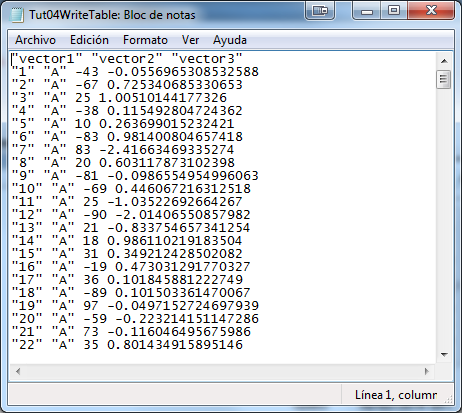
\includegraphics[width=8cm]{../fig/Tut04-18.png}
  \end{center}


  \item La primera dificultad es que R ha añadido una primera columna adicional con los números de las filas, que en Calc aparecen en la columna {\tt A} (eso, además, hace que los nombres de las variables queden descolocados), como se ve en esta figura.
  \begin{center}
  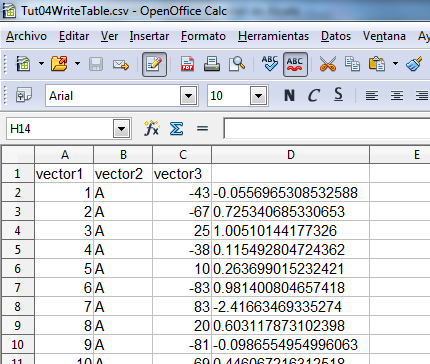
\includegraphics[width=10cm]{../fig/Tut04-19.png}
  \end{center}
  Pero, además, los elementos de la tercera columna usan puntos (en lugar de comas) como separadores decimales. A Calc, en su versión en español, eso le hace pensar que no se trata de números. Y si intentas calcular la media (recuerda usar la función {\tt PROMEDIO}) aparecerá un mensaje de error.

  \item El fichero {\tt Tut04WriteTable2.csv}, tras abrirlo con Calc y calcular la media de la tercera columna (en la celda {\tt E3}), muestra este aspecto:
  \begin{center}
  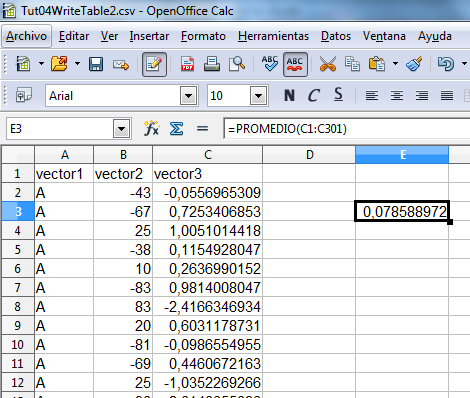
\includegraphics[width=10cm]{../fig/Tut04-20.png}
  \end{center}
  La media, calculada por Calc, se puede comprobar con R de cualquiera de estas dos formas (una usa el vector {\tt vector3} y la otra la tercera columna del {\tt data.frame}):
\begin{knitrout}
\definecolor{shadecolor}{rgb}{0.969, 0.969, 0.969}\color{fgcolor}\begin{kframe}
\begin{alltt}
\hlkwd{mean}\hlstd{(vector3)}
\end{alltt}
\begin{verbatim}
## [1] 0.0786
\end{verbatim}
\begin{alltt}
\hlkwd{mean}\hlstd{(Tut04WriteTable[,}\hlnum{3}\hlstd{])}
\end{alltt}
\begin{verbatim}
## [1] 0.0786
\end{verbatim}
\end{kframe}
\end{knitrout}


%%####################################################
%% Adicionales



\end{enumerate}


\paragraph{\bf $\bullet$ Ejercicio \ref{tut04:ejercicio06}, pág. \pageref{tut04:ejercicio06}}
\label{tut04:ejercicio06:sol}\quad\\

\begin{knitrout}
\definecolor{shadecolor}{rgb}{0.969, 0.969, 0.969}\color{fgcolor}\begin{kframe}
\begin{alltt}
\hlkwd{colnames}\hlstd{(satelitesGalileanos)} \hlkwb{=} \hlkwd{c}\hlstd{(}\hlstr{"nombres"}\hlstd{,} \hlstr{"diametrosKm"}\hlstd{,} \hlstr{"periodoOrbital"}\hlstd{)}
\hlkwd{head}\hlstd{(satelitesGalileanos)}
\end{alltt}
\begin{verbatim}
##     nombres diametrosKm periodoOrbital
## 1        Io        3643           1.77
## 2    Europa        3122           3.55
## 3 Ganimedes        5262           7.16
## 4   Calisto        4821          16.69
\end{verbatim}
\end{kframe}
\end{knitrout}
El resultado de {\tt dim} es:
\begin{knitrout}
\definecolor{shadecolor}{rgb}{0.969, 0.969, 0.969}\color{fgcolor}\begin{kframe}
\begin{alltt}
\hlkwd{dim}\hlstd{(satelitesGalileanos)}
\end{alltt}
\begin{verbatim}
## [1] 4 3
\end{verbatim}
\end{kframe}
\end{knitrout}
Es decir, un vector con el número de filas y columnas del {\tt data.frame}.

\paragraph{\bf $\bullet$ Ejercicio \ref{tut04:ejercicio07}, pág. \pageref{tut04:ejercicio07}}
\label{tut04:ejercicio07:sol}\quad\\

\begin{enumerate}
  \item El código para la primera parte es:
\begin{knitrout}
\definecolor{shadecolor}{rgb}{0.969, 0.969, 0.969}\color{fgcolor}\begin{kframe}
\begin{alltt}
\hlstd{traspuesta} \hlkwb{=} \hlkwd{t}\hlstd{(matrizDatos)}
\hlkwd{write.table}\hlstd{(traspuesta,} \hlkwc{file}\hlstd{=}\hlstr{"../datos/Traspuesta.csv"}\hlstd{,}
    \hlkwc{row.names} \hlstd{=} \hlnum{FALSE}\hlstd{,} \hlkwc{col.names}\hlstd{=}\hlnum{FALSE}\hlstd{,} \hlkwc{sep}\hlstd{=}\hlstr{" "}\hlstd{)}
\end{alltt}
\end{kframe}
\end{knitrout}
    Hemos dividido la función {\tt write.table} en dos líneas, para ajustarla al ancho de página.

  \item Para la segunda parte empezamos por leer el fichero en un data.frame, que vamos a llamar igual que el fichero (es una costumbre que a menudo resulta útil), salvo por el cambio de {\tt -} a {\tt \_}, porque el guión alto {\tt -} representa la resta en R, y no se puede usar en nombres de objetos:
\begin{knitrout}
\definecolor{shadecolor}{rgb}{0.969, 0.969, 0.969}\color{fgcolor}\begin{kframe}
\begin{alltt}
\hlstd{Tut04_3000datos} \hlkwb{=} \hlkwd{read.table}\hlstd{(}\hlkwc{file}\hlstd{=}\hlstr{"../datos/Tut04-3000datos.csv"}\hlstd{,} \hlkwc{header}\hlstd{=}\hlnum{FALSE}\hlstd{,} \hlkwc{sep}\hlstd{=}\hlstr{" "}\hlstd{)}
\end{alltt}
\end{kframe}
\end{knitrout}

  Una vez hecho esto, convertimos el {\tt data.frame} en una matriz:
\begin{knitrout}
\definecolor{shadecolor}{rgb}{0.969, 0.969, 0.969}\color{fgcolor}\begin{kframe}
\begin{alltt}
\hlstd{matriz3000Datos} \hlkwb{=} \hlkwd{as.matrix}\hlstd{(Tut04_3000datos)}
\hlkwd{head}\hlstd{(matriz3000Datos,} \hlnum{10}\hlstd{)}
\end{alltt}
\begin{verbatim}
##       V1 V2 V3 V4 V5
##  [1,] 81 21  6 40 43
##  [2,] 60 62 34 24 35
##  [3,] 60 35 37  7 63
##  [4,] 13 46 67 76 63
##  [5,] 69 72 94 83  9
##  [6,] 43 70 60 69 59
##  [7,] 40 81 17 73  2
##  [8,] 53 26 50 54 71
##  [9,] 13 33  9 22 82
## [10,] 12 44 60 55 45
\end{verbatim}
\end{kframe}
\end{knitrout}
  Para convertirlo en un vector, recorriendo la matriz por filas, vamos a usar lo que aprendimos en la Sección \ref{tut03-tut03:subsec:CaminoVueltaMatricesVectores} (pág. \pageref{tut03-tut03:subsec:CaminoVueltaMatricesVectores}) del Tutorial03. Mostramos sólo los primeros $20$ elementos del vector resultante:
\begin{knitrout}
\definecolor{shadecolor}{rgb}{0.969, 0.969, 0.969}\color{fgcolor}\begin{kframe}
\begin{alltt}
\hlkwd{head}\hlstd{(}\hlkwd{as.vector}\hlstd{(}\hlkwd{t}\hlstd{(matriz3000Datos)),} \hlnum{20}\hlstd{)}
\end{alltt}
\begin{verbatim}
##  [1] 81 21  6 40 43 60 62 34 24 35 60 35 37  7 63 13 46 67 76 63
\end{verbatim}
\end{kframe}
\end{knitrout}
  Finalmente para guardarlo en un fichero {\tt csv} puedes usar {\tt cat} (que ya conoces de anteriores tutoriales) o puedes usar {\tt write.table} así:
\begin{knitrout}
\definecolor{shadecolor}{rgb}{0.969, 0.969, 0.969}\color{fgcolor}\begin{kframe}
\begin{alltt}
\hlkwd{write.table}\hlstd{(}\hlkwd{as.vector}\hlstd{(}\hlkwd{t}\hlstd{(matriz3000Datos)),} \hlkwc{file}\hlstd{=}\hlstr{"../datos/Tut04-3000datos-solucion.csv"}\hlstd{,}
        \hlkwc{row.names}\hlstd{=}\hlnum{FALSE}\hlstd{,} \hlkwc{col.names}\hlstd{=}\hlnum{FALSE}\hlstd{)}
\end{alltt}
\end{kframe}
\end{knitrout}

\end{enumerate}

\paragraph{\bf $\bullet$ Ejercicio \ref{tut04:ejercicio08}, pág. \pageref{tut04:ejercicio08}}
\label{tut04:ejercicio08:sol}\quad\\

\begin{knitrout}
\definecolor{shadecolor}{rgb}{0.969, 0.969, 0.969}\color{fgcolor}\begin{kframe}
\begin{alltt}
\hlstd{(bolaUrna2} \hlkwb{=} \hlkwd{sample}\hlstd{(} \hlkwd{c}\hlstd{(}\hlstr{"blanca"}\hlstd{,}\hlstr{"negra"}\hlstd{),} \hlnum{1}\hlstd{,} \hlkwc{prob}\hlstd{=}\hlkwd{c}\hlstd{(}\hlnum{4}\hlstd{,}\hlnum{3}\hlstd{) ))}
\end{alltt}
\begin{verbatim}
## [1] "negra"
\end{verbatim}
\end{kframe}
\end{knitrout}

\paragraph{\bf $\bullet$ Ejercicio \ref{tut04:ejercicio09}, pág. \pageref{tut04:ejercicio09}}
\label{tut04:ejercicio09:sol}\quad\\

Los valores de {\tt cuenta} y {\tt k} se alternan en la salida. Ya aprenderemos a presentarlos un poco mejor.
\begin{knitrout}
\definecolor{shadecolor}{rgb}{0.969, 0.969, 0.969}\color{fgcolor}\begin{kframe}
\begin{alltt}
    \hlstd{cuenta}\hlkwb{=}\hlnum{0}
    \hlkwa{for}\hlstd{(k} \hlkwa{in} \hlnum{1}\hlopt{:}\hlnum{10}\hlstd{)\{}
        \hlcom{# Cuerpo del bucle (entre las dos llaves)}
        \hlstd{cuenta} \hlkwb{=} \hlstd{cuenta} \hlopt{+} \hlnum{3}
        \hlkwd{print}\hlstd{(cuenta)}
        \hlkwd{print}\hlstd{(k)}
    \hlstd{\}}
\end{alltt}
\begin{verbatim}
## [1] 3
## [1] 1
## [1] 6
## [1] 2
## [1] 9
## [1] 3
## [1] 12
## [1] 4
## [1] 15
## [1] 5
## [1] 18
## [1] 6
## [1] 21
## [1] 7
## [1] 24
## [1] 8
## [1] 27
## [1] 9
## [1] 30
## [1] 10
\end{verbatim}
\begin{alltt}
    \hlstd{cuenta}
\end{alltt}
\begin{verbatim}
## [1] 30
\end{verbatim}
\end{kframe}
\end{knitrout}

\paragraph{\bf $\bullet$ Ejercicio \ref{tut04:ejercicio10}, pág. \pageref{tut04:ejercicio10}}
\label{tut04:ejercicio10:sol}\quad\\

\begin{enumerate}
  \item Aquí puedes ver el resultado de tres ejecuciones del código, todas con $n=10000$:
\begin{knitrout}
\definecolor{shadecolor}{rgb}{0.969, 0.969, 0.969}\color{fgcolor}\begin{kframe}
\begin{verbatim}
## bola
##     b     n 
## 0.258 0.743
\end{verbatim}
\end{kframe}
\end{knitrout}
\begin{knitrout}
\definecolor{shadecolor}{rgb}{0.969, 0.969, 0.969}\color{fgcolor}\begin{kframe}
\begin{verbatim}
## bola
##     b     n 
## 0.251 0.749
\end{verbatim}
\end{kframe}
\end{knitrout}
\begin{knitrout}
\definecolor{shadecolor}{rgb}{0.969, 0.969, 0.969}\color{fgcolor}\begin{kframe}
\begin{verbatim}
## bola
##     b     n 
## 0.250 0.750
\end{verbatim}
\end{kframe}
\end{knitrout}

      \item El código modificado es este:
\begin{knitrout}
\definecolor{shadecolor}{rgb}{0.969, 0.969, 0.969}\color{fgcolor}\begin{kframe}
\begin{alltt}
\hlcom{# Empezamos lanzando un dado n veces.}
\hlstd{n} \hlkwb{=} \hlnum{10}
\hlstd{dado} \hlkwb{=} \hlkwd{sample}\hlstd{(}\hlnum{1}\hlopt{:}\hlnum{6}\hlstd{, n,} \hlkwc{replace}\hlstd{=}\hlnum{TRUE}\hlstd{)}

\hlcom{# El proceso ahora depende de si el dado es o no menor que 5}
\hlstd{bola}\hlkwb{=}\hlkwd{c}\hlstd{()}
\hlkwa{for}\hlstd{(k} \hlkwa{in} \hlnum{1}\hlopt{:}\hlstd{n)\{}
  \hlkwa{if}\hlstd{(dado[k]} \hlopt{<} \hlnum{5}\hlstd{)\{}
      \hlcom{#Se ha elegido la urna 1.}
      \hlcom{#Estas instrucciones (hasta la linea con else) se usan si dado<5}
      \hlcom{#print("Usamos una urna con 3 bolas blancas y 5 negras")}
      \hlstd{bola} \hlkwb{=} \hlkwd{c}\hlstd{(bola,} \hlkwd{sample}\hlstd{(}\hlkwd{c}\hlstd{(}\hlstr{"b"}\hlstd{,}\hlstr{"n"}\hlstd{),} \hlnum{1}\hlstd{,} \hlkwc{prob}\hlstd{=}\hlkwd{c}\hlstd{(}\hlnum{1}\hlstd{,}\hlnum{9}\hlstd{)) )}
  \hlstd{\}} \hlkwa{else} \hlstd{\{}
    \hlcom{#Se ha elegido la urna 2.}
    \hlcom{#Estas instrucciones (hasta la llave) se usan si dado>=5}
    \hlcom{#print("Usamos una urna con 7 bolas blancas y 3 negras")}
      \hlstd{bola} \hlkwb{=} \hlkwd{c}\hlstd{(bola,} \hlkwd{sample}\hlstd{(}\hlkwd{c}\hlstd{(}\hlstr{"b"}\hlstd{,}\hlstr{"n"}\hlstd{),} \hlnum{1}\hlstd{,} \hlkwc{prob}\hlstd{=}\hlkwd{c}\hlstd{(}\hlnum{4}\hlstd{,}\hlnum{3}\hlstd{)) )}
  \hlstd{\}}
  \hlkwd{print}\hlstd{(}\hlstr{"-----------------------------------------"}\hlstd{)}
  \hlkwd{print}\hlstd{(}\hlkwd{c}\hlstd{(}\hlstr{" dado ="}\hlstd{, dado[k]) )}
  \hlkwd{print}\hlstd{(}\hlkwd{c}\hlstd{(}\hlstr{"k = "}\hlstd{, k))}
  \hlkwd{print}\hlstd{(bola)}
\hlstd{\}}
\hlcom{# Y al final, miramos la tabla de frecuencias relativas.}
\hlkwd{table}\hlstd{(bola)} \hlopt{/} \hlkwd{length}\hlstd{(bola)}
\end{alltt}
\end{kframe}
\end{knitrout}
    Puedes ver que hemos cambiado $n=10$, y que hemos añadido un grupo de sentencias con la función {\tt print}, dentro del bucle {\tt for} pero fuera del condicional {\tt if/else}. El resultado de esas modificaciones es este:
\begin{knitrout}
\definecolor{shadecolor}{rgb}{0.969, 0.969, 0.969}\color{fgcolor}\begin{kframe}
\begin{verbatim}
## [1] "-----------------------------------------"
## [1] " dado =" "2"      
## [1] "k = " "1"   
## [1] "b"
## [1] "-----------------------------------------"
## [1] " dado =" "6"      
## [1] "k = " "2"   
## [1] "b" "n"
## [1] "-----------------------------------------"
## [1] " dado =" "4"      
## [1] "k = " "3"   
## [1] "b" "n" "b"
## [1] "-----------------------------------------"
## [1] " dado =" "4"      
## [1] "k = " "4"   
## [1] "b" "n" "b" "n"
## [1] "-----------------------------------------"
## [1] " dado =" "3"      
## [1] "k = " "5"   
## [1] "b" "n" "b" "n" "n"
## [1] "-----------------------------------------"
## [1] " dado =" "1"      
## [1] "k = " "6"   
## [1] "b" "n" "b" "n" "n" "n"
## [1] "-----------------------------------------"
## [1] " dado =" "4"      
## [1] "k = " "7"   
## [1] "b" "n" "b" "n" "n" "n" "n"
## [1] "-----------------------------------------"
## [1] " dado =" "6"      
## [1] "k = " "8"   
## [1] "b" "n" "b" "n" "n" "n" "n" "b"
## [1] "-----------------------------------------"
## [1] " dado =" "3"      
## [1] "k = " "9"   
## [1] "b" "n" "b" "n" "n" "n" "n" "b" "n"
## [1] "-----------------------------------------"
## [1] " dado =" "5"      
## [1] "k = " "10"  
##  [1] "b" "n" "b" "n" "n" "n" "n" "b" "n" "n"
## bola
##   b   n 
## 0.3 0.7
\end{verbatim}
\end{kframe}
\end{knitrout}
    Hemos usado un par de veces un ``truco'' para indicar cual es la variable que se muestra. Por ejemplo, en la línea de código:
\begin{knitrout}
\definecolor{shadecolor}{rgb}{0.969, 0.969, 0.969}\color{fgcolor}\begin{kframe}
\begin{alltt}
\hlkwd{print}\hlstd{(}\hlkwd{c}\hlstd{(}\hlstr{"k = "}\hlstd{, k))}
\end{alltt}
\end{kframe}
\end{knitrout}
    Al usar {\tt c("k = ", k)} estamos construyendo un vector que contiene una mezcla de números y texto. Es muy posible que no lo recuerdes, pero en la Sección \ref{tut02-tut02:subsec:Vectores} del Tutorial02 hemos comentado brevemente que en estos casos, R convierte todos los elementos del vector en cadenas alfanuméricas. El resultado dista todavía mucho de lo que se puede conseguir (¡todas esas comillas!), pero es un primer paso.

    Naturalmente, en este caso, con $n$ tan pequeño, las frecuencias se parecen bastante menos a las que predice la teoría.

\end{enumerate}






%#########################################################################################
%#########################################################################################
\vspace{2cm} \hrule
\quad\\
Fin del Tutorial-04. ¡Gracias por la atención!

%\newpage
%\addcontentsline{toc}{section}{Guía de trabajo.}
%\includepdf[pages={1-},scale=0.90]{04-GuiaDeTrabajo.pdf}

\end{document}
